\documentclass[pdflatex,sn-mathphys-num]{sn-jnl}%

%%%% Standard Packages
\usepackage{graphicx}%
\usepackage{multirow}%
\usepackage{amsmath,amssymb,amsfonts}%
\usepackage{amsthm}%
\usepackage{mathrsfs}%
\usepackage[title]{appendix}%
\usepackage{xcolor}%
\usepackage{textcomp}%
\usepackage{manyfoot}%
\usepackage{booktabs}%
\usepackage{algorithm}%
\usepackage{algorithmicx}%
\usepackage{algpseudocode}%
\usepackage{listings}%
\usepackage{subcaption}%
\usepackage{array}%
\usepackage{placeins}%
\usepackage{claims}%
\showclaimsfalse
% Generated by oran_causal.analysis.paper_values from spec/values.toml and data/records.
% Do not edit: run `uv run python -m oran_causal.analysis.paper_values`.
\defval{appa.prior.directed}{33}
\defval{br.pcorr_eq.recall}{0.72}
\defval{br.pcorr_native.recall}{0.69}
\defval{s1.attr.declared}{13}
\defval{s1.attr.true}{12}
\defval{s1.ex.confirmed}{26}
\defval{s1.ex.n_exists}{43}
\defval{s1.far.total}{20}
\defval{s1.far.true}{8}
\defval{s1.gt.dbl.int.prec}{0.88}
\defval{s1.gt.dbl.int.rec}{0.35}
\defval{s1.gt.dbl.pmrt.prec}{0.59}
\defval{s1.gt.dbl.pmrt.rec}{0.80}
\defval{s1.gt.dbl.qacm.prec}{0.80}
\defval{s1.gt.dbl.qacm.rec}{0.40}
\defval{s1.gt.dbl.shap.prec}{0.75}
\defval{s1.gt.dbl.shap.rec}{0.60}
\defval{s1.gt.dbl.tt.prec}{0.83}
\defval{s1.gt.dbl.tt.rec}{0.25}
\defval{s1.gt.episodes}{40}
\defval{s1.gt.half.prec}{1.00}
\defval{s1.gt.hypotheses}{60}
\defval{s1.k0.binom_level}{0.01}
\defval{s1.k0.binom_tail}{0.03}
\defval{s1.k0.m}{60}
\defval{s1.k0.n_reject}{7}
\defval{s1.k0.tail3}{0.030}
\defval{s1.k0n.fam_max}{0.060}
\defval{s1.k0n.fam_min}{0.047}
\defval{s1.k0n.rate}{0.053}
\defval{s1.map.corr.placebo}{3}
\defval{s1.map.corr.prec}{0.86}
\defval{s1.map.corr.rec}{0.21}
\defval{s1.map.corr.wrong}{1}
\defval{s1.map.gby.placebo}{13}
\defval{s1.map.gby.prec}{0.59}
\defval{s1.map.gby.rec}{0.76}
\defval{s1.map.gby.wrong}{6}
\defval{s1.map.gr.placebo}{1}
\defval{s1.map.gr.prec}{0.69}
\defval{s1.map.gr.rec}{0.62}
\defval{s1.map.gr.wrong}{4}
\defval{s1.map.int.placebo}{6}
\defval{s1.map.int.prec}{0.88}
\defval{s1.map.int.rec}{0.24}
\defval{s1.map.int.wrong}{0}
\defval{s1.map.pmrt.placebo}{0}
\defval{s1.map.pmrt.prec}{0.92}
\defval{s1.map.pmrt.rec}{0.79}
\defval{s1.map.pmrt.wrong}{0}
\defval{s1.map.qacm.placebo}{5}
\defval{s1.map.qacm.prec}{0.89}
\defval{s1.map.qacm.rec}{0.28}
\defval{s1.map.qacm.wrong}{0}
\defval{s1.map.shap.placebo}{8}
\defval{s1.map.shap.prec}{0.93}
\defval{s1.map.shap.rec}{0.48}
\defval{s1.map.shap.wrong}{0}
\defval{s1.map.tt.placebo}{6}
\defval{s1.map.tt.prec}{1.00}
\defval{s1.map.tt.rec}{0.21}
\defval{s1.map.tt.wrong}{1}
\defval{s1.null.ci.hi}{0.29}
\defval{s1.null.ci.lo}{0.043}
\defval{s1.null.count}{21}
\defval{s1.null.open.ci.hi}{0.16}
\defval{s1.null.open.ci.lo}{0.017}
\defval{s1.null.open.count}{12}
\defval{s1.null.open.rate}{0.075}
\defval{s1.null.rate}{0.15}
\defval{s1.p2.gby.wins120}{4}
\defval{s1.p2.gby.wins60}{2}
\defval{s1.p2.n120}{5}
\defval{s1.p2.n60}{10}
\defval{s1.placebo.granger_by}{13}
\defval{s1.pmrt.declared}{28}
\defval{s1.pmrt.indet}{3}
\defval{s1.pmrt.precision}{0.92}
\defval{s1.pmrt.recall}{0.79}
\defval{s2.assoc.ratio_max}{5.4}
\defval{s2.assoc.ratio_min}{4.5}
\defval{s2.attr.declared}{7}
\defval{s2.dec.aa.dn}{-0.22}
\defval{s2.dec.aa.dn_hi}{-0.14}
\defval{s2.dec.aa.dn_lo}{-0.30}
\defval{s2.dec.aa.dr}{$-0.22$}
\defval{s2.dec.aa.dr_hi}{$-0.14$}
\defval{s2.dec.aa.dr_lo}{$-0.30$}
\defval{s2.dec.aa.rcv}{0.00}
\defval{s2.dec.aa.ret}{1.00}
\defval{s2.dec.aa.rlf}{1.00}
\defval{s2.dec.aa.rlf_hi}{1.00}
\defval{s2.dec.aa.rlf_lo}{1.00}
\defval{s2.dec.gt.dn}{0.02}
\defval{s2.dec.gt.dn_hi}{0.09}
\defval{s2.dec.gt.dn_lo}{-0.04}
\defval{s2.dec.gt.dr}{$+0.02$}
\defval{s2.dec.gt.dr_hi}{$0.09$}
\defval{s2.dec.gt.dr_lo}{$-0.04$}
\defval{s2.dec.gt.rcv}{0.24}
\defval{s2.dec.gt.ret}{1.32}
\defval{s2.dec.gt.rlf}{1.01}
\defval{s2.dec.gt.rlf_hi}{1.09}
\defval{s2.dec.gt.rlf_lo}{0.94}
\defval{s2.dec.ns.rcv}{0.22}
\defval{s2.dec.ns.ret}{1.18}
\defval{s2.dec.ns.rlf}{0.99}
\defval{s2.dec.ns.rlf_hi}{1.04}
\defval{s2.dec.ns.rlf_lo}{0.94}
\defval{s2.dec.pmrt.dn}{0.25}
\defval{s2.dec.pmrt.dn_hi}{0.36}
\defval{s2.dec.pmrt.dn_lo}{0.14}
\defval{s2.dec.pmrt.dr}{$+0.25$}
\defval{s2.dec.pmrt.dr_hi}{$0.36$}
\defval{s2.dec.pmrt.dr_lo}{$0.14$}
\defval{s2.dec.pmrt.rcv}{0.47}
\defval{s2.dec.pmrt.ret}{1.67}
\defval{s2.dec.pmrt.rlf}{1.31}
\defval{s2.dec.pmrt.rlf_hi}{1.56}
\defval{s2.dec.pmrt.rlf_lo}{1.10}
\defval{s2.dec.seeds}{160}
\defval{s2.defer.ptx_up.gt}{2\,370}
\defval{s2.defer.ptx_up.pmrt}{8\,674}
\defval{s2.ex.confirmed}{22}
\defval{s2.ex.n_exists}{40}
\defval{s2.far.true}{9}
\defval{s2.gt.dbl.pmrt.prec}{0.73}
\defval{s2.gt.half.prec}{1.00}
\defval{s2.k0.m}{60}
\defval{s2.k0.n_reject}{0}
\defval{s2.k0n.fam_max}{0.063}
\defval{s2.k0n.fam_min}{0.038}
\defval{s2.k0n.rate}{0.050}
\defval{s2.map.corr.placebo}{8}
\defval{s2.map.corr.prec}{0.80}
\defval{s2.map.corr.rec}{0.28}
\defval{s2.map.corr.wrong}{2}
\defval{s2.map.gby.placebo}{29}
\defval{s2.map.gby.prec}{0.54}
\defval{s2.map.gby.rec}{0.76}
\defval{s2.map.gby.wrong}{6}
\defval{s2.map.gr.placebo}{19}
\defval{s2.map.gr.prec}{0.60}
\defval{s2.map.gr.rec}{0.62}
\defval{s2.map.gr.wrong}{6}
\defval{s2.map.int.placebo}{1}
\defval{s2.map.int.prec}{0.80}
\defval{s2.map.int.rec}{0.14}
\defval{s2.map.int.wrong}{0}
\defval{s2.map.pmrt.placebo}{0}
\defval{s2.map.pmrt.prec}{0.86}
\defval{s2.map.pmrt.rec}{0.62}
\defval{s2.map.pmrt.wrong}{0}
\defval{s2.map.qacm.placebo}{0}
\defval{s2.map.qacm.prec}{0.83}
\defval{s2.map.qacm.rec}{0.17}
\defval{s2.map.qacm.wrong}{0}
\defval{s2.map.shap.placebo}{0}
\defval{s2.map.shap.prec}{0.80}
\defval{s2.map.shap.rec}{0.28}
\defval{s2.map.shap.wrong}{0}
\defval{s2.map.tt.placebo}{22}
\defval{s2.map.tt.prec}{0.63}
\defval{s2.map.tt.rec}{0.17}
\defval{s2.map.tt.wrong}{0}
\defval{s2.placebo.granger_by}{29}
\defval{s2.plc.rec_max}{0.55}
\defval{s2.pmrt.declared}{22}
\defval{s2.pmrt.indet}{1}
\defval{s2.ptx_nbr_rlf.primary_p}{0.49}
\defval{s3.dec.aa.dn}{-0.26}
\defval{s3.dec.aa.dn_hi}{-0.17}
\defval{s3.dec.aa.dn_lo}{-0.34}
\defval{s3.dec.aa.dr}{$-0.26$}
\defval{s3.dec.aa.dr_hi}{$-0.17$}
\defval{s3.dec.aa.dr_lo}{$-0.34$}
\defval{s3.dec.aa.rcv}{0.00}
\defval{s3.dec.aa.ret}{1.00}
\defval{s3.dec.aa.rlf}{1.00}
\defval{s3.dec.aa.rlf_hi}{1.00}
\defval{s3.dec.aa.rlf_lo}{1.00}
\defval{s3.dec.gt.dn}{-0.04}
\defval{s3.dec.gt.dn_hi}{0.03}
\defval{s3.dec.gt.dn_lo}{-0.10}
\defval{s3.dec.gt.dr}{$-0.04$}
\defval{s3.dec.gt.dr_hi}{$0.03$}
\defval{s3.dec.gt.dr_lo}{$-0.10$}
\defval{s3.dec.gt.rcv}{0.22}
\defval{s3.dec.gt.ret}{1.29}
\defval{s3.dec.gt.rlf}{0.94}
\defval{s3.dec.gt.rlf_hi}{0.97}
\defval{s3.dec.gt.rlf_lo}{0.90}
\defval{s3.dec.ns.rcv}{0.26}
\defval{s3.dec.ns.ret}{1.15}
\defval{s3.dec.ns.rlf}{0.96}
\defval{s3.dec.ns.rlf_hi}{0.99}
\defval{s3.dec.ns.rlf_lo}{0.93}
\defval{s3.dec.pmrt.dn}{0.00}
\defval{s3.dec.pmrt.dn_hi}{0.00}
\defval{s3.dec.pmrt.dn_lo}{0.00}
\defval{s3.dec.pmrt.dr}{$0.00$}
\defval{s3.dec.pmrt.dr_hi}{$0.00$}
\defval{s3.dec.pmrt.dr_lo}{$0.00$}
\defval{s3.dec.pmrt.rcv}{0.26}
\defval{s3.dec.pmrt.ret}{1.15}
\defval{s3.dec.pmrt.rlf}{0.96}
\defval{s3.dec.pmrt.rlf_hi}{0.99}
\defval{s3.dec.pmrt.rlf_lo}{0.93}
\defval{s3.dec.seeds}{160}
\defval{s3.gate.dev_episodes}{40}
\defval{s3.gate.g_rlf}{35.025}
\defval{s3.gate.g_v}{19\,953.65}
\defval{s3.mgpmrt.dr}{$-0.06$}
\defval{s3.mgpmrt.rlf}{1.05}
\defval{s4.c1.r2_max}{0.94}
\defval{s4.c1.r2_min}{0.33}
\defval{s4.cdl.conditions}{30}
\defval{s4.cdl.invalid}{9}
\defval{s4.conf.corr_all}{0.77}
\defval{s4.conf.corr_min}{1.00}
\defval{s4.conf.gbm_max}{0.06}
\defval{s4.conf.gbm_min}{0.02}
\defval{s4.conf.pcorr_all}{0.056}
\defval{s4.conf.rcot2_all}{0.23}
\defval{s4.dither.max}{0.054}
\defval{s4.dither.min}{0.042}
\defval{s4.e4.pcorr_eq.recall_24k}{0.90}
\defval{s4.e4.pmrtgbm.recall_max}{0.075}
\defval{x11.delta_dbl.changed}{16}
\defval{x11.delta_half.changed}{10}
\defval{x11.other.changed_max}{2}
\defval{x11.pmrt.sign_acc_min}{1.00}
\defval{x14.gby.wrong_s1}{24}
\defval{x14.gby.wrong_s2}{21}
\defval{x15.block_diff}{0.30}
\defval{x15.p.never_sleep}{0.17}
\defval{x15.p.noarb}{0.15}
\defval{x15.perm_p}{0.009}
\defval{x15.pooled.dr}{0.10}
\defval{x15.pooled.rlf}{1.18}
\defval{x15.r.never_sleep_s2}{0.22}
\defval{x15.r.never_sleep_s3}{0.26}
\defval{x15.rej.s2}{0.37}
\defval{x15.rej.s3}{0.35}
\defval{x15.sd.s2}{0.85}
\defval{x15.sd.s3}{1.1}
\defval{x15.trim.s2}{0.21}
\defval{x15.trim.s3}{0.041}
\defval{x16.gate.median_pct}{3.5}
\defval{x16.map.rel_max}{$+6.5$}
\defval{x16.map.rel_min}{$-2.9$}
\defval{x8.lim.1e3}{2 \times 10^{-3}}
\defval{x8.lim.2e4}{6 \times 10^{-4}}
\defval{x8.n_variants}{590}
\defval{x8.redraws}{9\,999}
\defval{x8.share.1e3}{7.9 \times 10^{-4}}
\defval{x8.share.2e4}{1.1 \times 10^{-4}}
\defval{x8.tol_pct}{7.5}
\defval{x8.variants_with_decl}{2}

%%%%

\theoremstyle{thmstyleone}%
\newtheorem{theorem}{Theorem}%
\newtheorem{proposition}[theorem]{Proposition}%
\newtheorem{corollary}{Corollary}%
\newtheorem{lemma}{Lemma}%

\theoremstyle{thmstyletwo}%
\newtheorem{example}{Example}%
\newtheorem{remark}{Remark}%

\theoremstyle{thmstylethree}%
\newtheorem{definition}{Definition}%

\raggedbottom

\renewcommand{\thesection}{S\arabic{section}}%
\renewcommand{\thetable}{S\arabic{table}}%
\renewcommand{\thefigure}{S\arabic{figure}}%
\renewcommand{\theequation}{S\arabic{equation}}%

\begin{document}

\title[Online Resource 1]{Online Resource 1\\[6pt]
\large Supplementary material for: Design-Based Causal Effect Maps for O-RAN xApp Conflicts}

\author*[1]{\fnm{First} \sur{Author}}\email{first.author@example.com}

\author[1]{\fnm{Second} \sur{Author}}\email{second.author@example.com}

\author[2]{\fnm{Third} \sur{Author}}\email{third.author@example.com}

\affil*[1]{\orgdiv{Department}, \orgname{Organization}, \orgaddress{\city{City}, \country{Country}}}

\affil[2]{\orgdiv{Department}, \orgname{Organization}, \orgaddress{\city{City}, \country{Country}}}

\abstract{This Online Resource supplements the article ``Design-Based Causal Effect Maps for O-RAN xApp Conflicts''.
It contains the weight construction and the declaration rules (Section~\ref{esm:method}), the theorem statements with proof
ideas (Section~\ref{esm:theory}), the simulation set-up (Section~\ref{esm:setup}), and the supplementary results on
discovery (Section~\ref{esm:discovery}), decisions (Section~\ref{esm:decision}), controlled environments
(Section~\ref{esm:envs}) and the bridging analysis (Section~\ref{esm:bridge}). Section, table and figure numbers without
an S refer to the article.}

\maketitle

\section{Method}
\label{esm:method}

Algorithm~1 of the article collects the steps of the test for one hypothesis, Table~\ref{tab:s_pipeline} the construction of the weight $w_u$ of unit $u$ for hypothesis $(f, r, k)$ (steps 1 to 7, fitted on training, the 480 earlier and 20 development episodes) and of the inputs of the declaration layer (step 8, which runs steps 1 to 7 on the 480 earlier episodes), and Table~\ref{tab:s_rules} the rules of the test and the referee.

\begin{table}[tbp]
\caption{Weight construction.}
\label{tab:s_pipeline}
\footnotesize
\setlength{\tabcolsep}{3pt}
\begin{tabular*}{\textwidth}{@{\extracolsep{\fill}}>{\raggedright}p{0.2\textwidth}>{\raggedright}p{0.6\textwidth}>{\raggedright\arraybackslash}p{0.15\textwidth}@{}}
\toprule
Step & What it does & Fitted on \\
\midrule
1 Target bins & KPI $k$ over the cells of $r$, at 0--30, 30--60, 60--90 and 90--150~s after opening & -- \\
2 Receiver slots & Own 1, neighbour 4, far 2 slots: cells whose load the family moved most get one each, the rest share one & training \\
3 Adjustment & Ridge prediction from pre-window bins, context and earlier units' centred modes; residual kept & training \\
4 Matched filter & Score $g_u$: step-3 residuals weighted by $\psi = \Sigma^{-1} \tilde\mu$, favouring bins with more effect and less noise $\Sigma$ (Ledoit--Wolf), where $\tilde\mu$ is the rank-one fit of the effect profile $\mu$: a one-signed profile over slots, taken from the family's effect on load, times a least-squares profile over the four bins; restricted to the bins present & training \\
5 Score centre & Subtracts $\bar g_u$, the running mean score of earlier units of the same episode and request direction, shrunk towards the mean over earlier units of that direction (20 pseudo-units) and the training mean (50 pseudo-units) & training and earlier units, online \\
6 Huber clip & Clips at a scale predicted at opening, giving $w_u$ & training \\
7 Orientation & $o$, see Table~\ref{tab:s_rules}; $z_{\mathrm{train}}$ is the $z$ of the plain 0--90~s total of the step-3 residuals & training \\
\midrule
8 Declaration weights & Roeder--Wasserman $\omega_j$ (Roeder and Wasserman 2009, Thm.~3.1; adapted to the BY step-up; floor and cap ours): floor 0.2, cap 5, mean 1; direction $d_j$, sign of $z$ where $|z| \ge 3$ (\val{appa.prior.directed} of 60) & the 480 earlier episodes \\
\botrule
\end{tabular*}
\end{table}

\begin{table}
\caption{Rules of the map-driven referee and of the test.}
\label{tab:s_rules}
\footnotesize
\setlength{\tabcolsep}{3pt}
\begin{tabular*}{\textwidth}{@{\extracolsep{\fill}}>{\raggedright}p{0.2\textwidth}>{\raggedright\arraybackslash}p{0.75\textwidth}@{}}
\toprule
Rule & Definition \\
\midrule
\multicolumn{2}{@{}l}{\textit{Test}} \\
Support & A hypothesis is tested only with at least 30 units, 5 accepted, 5 rejected and 3 episodes, at least 30 training units of its family, and an outcome defined for every unit \\
Orientation & $o$ is the sign of the rank-one fitted training effect $\tilde\mu$ over 0--90~s, set only if $|z_{\mathrm{train}}| \ge 2$; where $o$ is unset, the reported sign is that of the plain total of the residuals over 0--90~s \\
\midrule
\multicolumn{2}{@{}l}{\textit{Referee}} \\
Opening & A request opens a unit only if its parameter last changed longer ago than the actuator's minimum interval between changes; a rejecting unit rejects only requests in its opening direction \\
Effects & For a request of family $f$ and direction $d$, sums the direction-adjusted effects $\Delta_k = d \sum_r \beta(f, r, k)$ over the own, neighbour and far relations for each KPI $k$ \\
Harm & The request is judged on the first KPI with $\Delta_k \ne 0$ in the order protected-slice violations, service violations, RLFs; it is harmful if that $\Delta_k$ is positive, and otherwise accepted \\
Rejection & The request is costly if $\Delta_e > 0$ for energy; its pressure is the largest protected-UE below-floor fraction over the own and neighbour relations through which it is harmful, or zero without such a relation or report; a harmful request is rejected if it is costly or its pressure exceeds 0.05 \\
Guard conflict & A rejection is guard-conflicted when accepting would help the first nonzero guard KPI among service violations and RLFs; such a unit is rejected only if the previous unit of the same cell and family was accepted \\
Map coefficient & PMRT: the declaration's sign times the magnitude of the design slope, the declaration's sign kept where the two disagree; associational maps: the method's sign times the magnitude of the least-squares slope of the outcome on the logged mode, oriented by the request's direction \\
Gate certification & An undeclared guard edge is certified when the one-sided 90~\% upper bound of $h\beta$ is at most $\varepsilon(f, d, k)$; PMRT uses the design slope with its martingale standard error, associational maps the least-squares slope with an independent-error standard error, the oracle map a conservative bound from its stored 95~\% interval; $G_k$ and $N(f, d)$ are measured under accept-all on 40 development episodes \\
\bottomrule
\end{tabular*}
\end{table}

\FloatBarrier
\section{Theory}
\label{esm:theory}

Each result has its statement, a proof idea and the module and declaration of its machine-checked version in the
\texttt{proofs/} directory of the code repository.\footnote{Repository: oran-causal, directory \texttt{proofs/}.}
% TODO DOI
Lemma~\ref{lem:s_fresh}, Lemma~\ref{lem:s_exact}, the finite weighted Benjamini--Yekutieli bound and the gate budget are
fully machine-checked. Proposition~1 and Corollary~1 are machine-checked taking the martingale central limit theorem
of Hall and Heyde and the Lindeberg--Feller and P\'olya theorems as given. Lemma~\ref{lem:s_slope} and
Example~\ref{ex:s_adaptive} are machine-checked under the hypotheses stated.

\subsection{Setting}
\label{esm:setting}

Fix a hypothesis $(f, r, k)$. Let $Y_\xi$ be the target that a unit of $f$ with key $\xi$ (episode, cell, xApp, opening
second) would have; the sharp null states that every $Y_\xi$ is the same under any assignment of $f$'s modes. The draws
of family $f$ form a field $\{U_\xi\}$ of independent Uniform$(0, 1)$ variables, independent of $\mathcal{G}_0$, which
holds all other randomness. Unit $u$ of $f$, in information order, has key $\xi_u$ and mode
$W_u = \text{accept}$ if and only if $U_{\xi_u} < \pi_u$, and
$\mathcal{G}_u = \mathcal{G}_0 \vee \sigma(U_{\xi_1}, \dots, U_{\xi_u})$. Assumption (A4) states formally that, as the
number of episodes $n$ grows, there are constants $s_n \to \infty$ with $\sigma^2 / s_n^2 \to \eta^2$ in probability,
$0 < \eta^2 < \infty$ almost surely, and $\max_u |w_u| / s_n \to 0$ in probability.

\subsection{Statements and proof ideas}
\label{esm:statements}

\begin{lemma}[Fresh draws]
\label{lem:s_fresh}
If $\xi_u$ and $\pi_u$ are $\mathcal{G}_{u-1}$-measurable and $\xi_u$ differs from $\xi_1, \dots, \xi_{u-1}$, then
$U_{\xi_u}$ is Uniform$(0, 1)$ and independent of $\mathcal{G}_{u-1}$, so
$\Pr(W_u = \text{accept} \mid \mathcal{G}_{u-1}) = \pi_u$.
\end{lemma}
\noindent\emph{Proof idea.} On the event $\{\xi_u = \xi\}$ the recursion that builds the earlier keys never reads
$U_\xi$, so every event of $\mathcal{G}_{u-1}$ intersected with it is independent of $U_\xi$; summing over the countably
many keys gives the claim. \emph{Lean:} \texttt{OranCausal.Fresh.fresh\_draw}.

\begin{proposition}[Asymptotic validity of PMRT, Proposition~1 of the article]
\label{prop:s_pmrt}
Under (A1) to (A3), $S$ is a martingale with predictable quadratic variation $\sigma^2$; under (A4) also, $z$ converges
to $\mathcal{N}(0, 1)$, the redraw distribution converges uniformly to $\Phi$ in probability, and for every fixed $B$
the p-value is asymptotically valid.
\end{proposition}
\noindent\emph{Proof idea.} The increments $v_u w_u$ are martingale differences whose conditional variances sum to
$\sigma^2$, so the martingale central limit theorem with a random limiting variance gives $z \to \mathcal{N}(0, 1)$. Given
the data the redraws are independent, so the Lindeberg--Feller and P\'olya theorems give the same limit uniformly. Given
the data, the redraw count is binomial, and mixing it over the uniform limit of the normal p-value gives a uniform law on
the grid $\{1/(B+1), \dots, 1\}$. \emph{Lean:} \texttt{OranCausal.Asymptotic.asymptotic\_rejection\_bound}, with the
martingale central limit theorem and the Lindeberg--Feller and P\'olya theorems as named hypotheses
(\texttt{HallHeyde}, \texttt{LindebergFellerPolya}).

\begin{lemma}[Exact case]
\label{lem:s_exact}
If, in addition to (A1) and (A2), the realised units, their order, $\mathrm{sgn}_u$, $\pi_u$ and $w_u$ are all
$\mathcal{G}_0$-measurable, then $\Pr(p \le t \mid \mathcal{G}_0) \le t$ for every $t \in [0, 1]$, every $n$ and every
$B$, and likewise for $p_d$.
\end{lemma}
\noindent\emph{Proof idea.} By the fresh-draw lemma the modes are independent with propensities $\pi_u$ given
$\mathcal{G}_0$, so the observed assignment and the $B$ redraws are exchangeable and the tie-inclusive Monte Carlo
p-value is valid. \emph{Lean:} \texttt{OranCausal.Exact.conditional\_iid\_rank\_valid}.

\begin{example}[Re-proposal alone breaks finite-sample validity]
\label{ex:s_adaptive}
Let $\pi_u = 0.5$, $\mathrm{sgn}_u = +1$, $o = +1$ and $w_1 = 1$. If unit 1 is rejected, the request is proposed again and
opens unit 2 with weight $w_2 = a > 1$; if it is accepted, there is no unit 2. Then, for every fixed
$t \in (1/2, 3/4)$, $\Pr(p_{+1} \le t) \to 3/4 > t$ as $B \to \infty$.
\end{example}
\noindent\emph{Proof idea.} The exact tail of the observed statistic is at most $1/2$ with probability $3/4$, while the
plus-one p-value estimates a tail of $1/2$ by a binomial count and tends to $1/2$; the redraws treat unit 2 as if it
existed whatever unit 1 received. \emph{Lean:}
\texttt{OranCausal.Counterexample.finite\_\allowbreak redraw\_\allowbreak rejection\_\allowbreak limit\_\allowbreak between\_\allowbreak half\_\allowbreak and\_\allowbreak three\_\allowbreak quarters}.

\begin{corollary}[Asymptotic false discovery rate, Corollary~1 of the article]
\label{cor:s_fdr}
Under (A1) to (A4) for every true sharp null, with weights $\omega_{n,j} \to \omega_j$ and directions fixed from
independent data, $\limsup_n \mathrm{FDR} \le (q/m) \sum_{j \in \mathcal{H}_0} \omega_j \le q$.
\end{corollary}
\noindent\emph{Proof idea.} Apply the finite bound at each $n$ with a slack that vanishes. For fixed $B$ the Monte Carlo
p-value takes values on the grid $k/(B+1)$, so the limit in Proposition~1 holds uniformly in $t$, which lets the
thresholds move with $n$. \emph{Lean:} \texttt{OranCausal.FDRAsymptotic.limsup\_fdr\_le\_const} (weights fixed in $n$)
and \texttt{limsup\_fdr\_le\_of\_tendsto} (weights convergent).

\begin{lemma}[Design slope]
\label{lem:s_slope}
Assume (A1) with the natural history $\mathcal{F}_{u-1}$, bounded outcomes, a bounded centre $\tilde y_u$ that is
$\mathcal{F}_{u-1}$-measurable, outcomes that close within their episode, at most $N_{\max}$ units per episode,
episodes appended in a fixed order, and $N / n$ bounded away from 0 and infinity with probability tending to one. Then
$\hat\beta - \sum_u \pi_u (1 - \pi_u)\, \mathrm{sgn}_u\, \tau_u^{\pi} / \sum_u \pi_u (1 - \pi_u) \to 0$ in probability;
for $\pi_u = 0.5$ the fraction is $\bar\tau_{\pi}$ and the estimator is the Horvitz--Thompson identity.
\end{lemma}
\noindent\emph{Proof idea.} The centred errors summed over an episode are bounded martingale differences over the
episodes, so a weak law (Chebyshev) gives the limit; at $\pi_u = 0.5$ the identity is algebra.
\emph{Lean:} \texttt{OranCausal.Slope.EpisodeDesign.corrected\_convergence}.

\begin{lemma}[Finite weighted BY bound]
\label{lem:s_by}
Let $m \ge 1$, $q \ge 0$, weights $w_j \ge 0$, thresholds $t_j(i) = q\, w_j\, i / (m c_m)$ with $c_m = \sum_{i=1}^m 1/i$,
and measurable p-values $p_j$. If the rejection set $S$ satisfies $p_j \le t_j(|S|)$ for every $j \in S$ and every true
null satisfies $\Pr(p_j \le t_j(i)) \le t_j(i) + \delta$ for $i = 1, \dots, m$, then, whatever the dependence between
the p-values, $\mathrm{FDR} \le (q/m) \sum_{j \in \mathcal{H}_0} w_j + |\mathcal{H}_0|\, \delta$.
\end{lemma}
\noindent\emph{Proof idea.} Each null's contribution to the FDR is bounded by an envelope of its distribution function
on the threshold grid, which the Benjamini--Yekutieli argument (Benjamini and Yekutieli 2001, proof of Thm.~1.3; Blanchard and Roquain
2008, Prop.~2.7 and Prop.~3.7) sums to $q\, w_j / m$ plus the slack.
\emph{Lean:} \texttt{OranCausal.StepUp.fdr\_le\_of\_selfConsistent}.

\begin{lemma}[Gate budget]
\label{lem:s_gate}
If a class has at most $\max\{N, 1\}$ units and each rejection moves a guard KPI by at most
$\varepsilon = 0.05\, G / (3 \max\{N, 1\})$ on each of the three relations, the guard ratio moves by at most $0.05$.
\end{lemma}
\noindent\emph{Proof idea.} Sum the movements over units and relations and divide by $G$.
\emph{Lean:} \texttt{OranCausal.GateBudget.additive\_guard\_budget}.

\FloatBarrier
\section{Simulation set-up}
\label{esm:setup}

Table~\ref{tab:s_params} gives the simulation and evaluation parameters, Table~\ref{tab:s_hyp} the knockout ground truth of the 60 hypotheses and Table~\ref{tab:s_armdef} the decision arms and metrics.

\begin{table}
\caption{Simulation and evaluation parameters.}
\label{tab:s_params}
\footnotesize
\setlength{\tabcolsep}{3pt}
\begin{tabular*}{\textwidth}{@{\extracolsep{\fill}}>{\raggedright}p{0.2\textwidth}>{\raggedright\arraybackslash}p{0.75\textwidth}@{}}
\toprule
Group & Value \\
\midrule
Network & 21 macro sectors on a seven-site hexagonal layout with wrap-around, inter-site distance 500~m; 3 co-channel picos; 300 UEs; 20~MHz carrier \\
Radio and energy & 3GPP TR 38.901 path loss with correlated shadowing and 3GPP antenna patterns; handover by A3 with time-to-trigger; radio-link failure by T310; EARTH power model, carrier shutdown for macro sectors, sleep for picos \\
Scheduler and timing & Slice-aware scheduler (dedicated low-latency pool, work-conserving protected minimum share, shared pool); tick 40~ms; delayed KPM reports; configuration changes take effect at the next tick; 120~s warm-up and 600~s scored time per episode \\
Surge scenario & Surge triples the file-arrival rate of the UEs within 250~m of a venue; offered load fills 40~\% of the PRBs with every xApp inactive \\
Slices and KPIs & Protected subset: 20~\% of the eMBB UEs, per-UE floor 2~Mb/s; LL UE-second violated above 100~ms head-of-line delay; eMBB UE-second violated when backlogged below 2~Mb/s; any UE-second in RLF or out of coverage \\
Decision unit & Hold 60~s; outcome window 90~s before and after opening \\
Test & $B = 9999$ redraws; training on 480 earlier and 20 development episodes \\
Gate calibration & 40 development episodes under accept-all; $G_{\mathrm{v}} = \val{s3.gate.g_v}$ violated UE-seconds, $G_{\mathrm{RLF}} = \val{s3.gate.g_rlf}$ RLFs \\
Ground truth & 90~s rollouts from the opening state, accepted and rejected, three reseeds; label threshold $\delta_k$ = 5~\% of the largest absolute mean of KPI $k$, floor 0.5 violated UE-seconds for protected-slice violations; unscored with fewer than 10 units or 3 episodes; 95~\% episode-cluster bootstrap \\
Intervals & Decision metrics: 90~\% paired seed-bootstrap, 10\,000 resamples; rates: 95~\% cluster bootstrap \\
\bottomrule
\end{tabular*}
\end{table}

\begin{table}[tbp]
\caption{Knockout ground truth of the 60 hypotheses, randomised logs.}
\label{tab:s_hyp}
% tab_system_hypotheses: generated by cddfig (figures/src/cddfig/figs/tab_system_hypotheses.py); do not edit.
% Sources: CDD-ORAN/scratchpad/e6_dev/decision/v4_analysis.json, CDD-ORAN/reports/2026-10-02-v4-pmrt-confounded-certsafe/figures_data.json
% Knockout ground truth of Study 1 (randomised logs); sign = accept-minus-reject effect of a request that raises the parameter (60 s mode contrast); TRUE 29, NULL 21, INDET 10.
% Needs \usepackage{booktabs} and the \verdict macro (sn-article.tex).
\setlength{\tabcolsep}{3pt}
\begin{tabular}{@{}l l c c c c c@{}}
\toprule
\shortstack[l]{Parameter\\(writer)} & Relation & \shortstack{protected-slice\\violations} & \shortstack{service\\violations} & \shortstack{radio-link\\failures} & energy & \shortstack{served\\load} \\
\midrule
carrier & own & true $-$ & true $-$ & indeterminate & true $+$ & null \\
(ES) & neighbour & indeterminate & null & indeterminate & indeterminate & null \\
 & far & indeterminate & null & indeterminate & null & null \\
\midrule
sleep & own & indeterminate & indeterminate & true $-$ & null & true $-$ \\
(ES) & neighbour & true $+$ & true $+$ & true $+$ & true $+$ & true $+$ \\
 & far & true $+$ & true $+$ & true $+$ & true $+$ & true $+$ \\
\midrule
ptx & own & true $+$ & true $+$ & true $+$ & true $+$ & true $+$ \\
(Power ES) & neighbour & true $-$ & true $-$ & true $-$ & true $-$ & true $-$ \\
 & far & indeterminate & true $-$ & indeterminate & true $-$ & true $-$ \\
\midrule
prot\_min & own & true $-$ & null & null & null & null \\
(Slice Guarantee) & neighbour & null & null & null & null & null \\
 & far & null & null & null & null & null \\
\bottomrule
\end{tabular}

\end{table}

Table~\ref{tab:s_baselines} lists the associational baselines. Each ran on the same unit table as PMRT and gave a score and a sign per hypothesis under the same support rule; on the confounded logs each tuned baseline also received a threshold calibrated on the placebo logs, which allows at most one placebo edge.

\begin{table}
\caption{Associational baselines.}
\label{tab:s_baselines}
\footnotesize
\setlength{\tabcolsep}{3pt}
\begin{tabular*}{\textwidth}{@{\extracolsep{\fill}}>{\raggedright}p{0.17\textwidth}>{\raggedright}p{0.5\textwidth}>{\raggedright\arraybackslash}p{0.26\textwidth}@{}}
\toprule
Baseline & Score & Threshold \\
\midrule
Correlation & Absolute Pearson correlation between the signed level and the change in the relation's KPI & Tuned \\
Granger & Test of the level's coefficient in a regression of the post-window KPI on its pre-window value and the signed level & Tuned; BY control at $q = 0.05$ (Granger~+~BY) \\
SHAP-GBDT & SHAP importance of the level in one gradient-boosted tree model per hypothesis, without the effect estimation of Sharma et al. & Tuned \\
Two-tower & Gate of a learned gated model between a parameter family and a target & Tuned \\
INT & Distance between the outcome distributions of accepted and rejected units (PACIFISTA) & Tuned \\
QACM & Predicted change of the KPI predictor of Wadud et al. fitted on the acted-on cell; never declares a neighbour or far edge & Tuned \\
\bottomrule
\end{tabular*}
\end{table}

\begin{table}[tbp]
\caption{Decision arms and metrics.}
\label{tab:s_armdef}
\footnotesize
\setlength{\tabcolsep}{3pt}
\begin{tabular*}{\textwidth}{@{\extracolsep{\fill}}>{\raggedright}p{0.24\textwidth}>{\raggedright\arraybackslash}p{0.7\textwidth}@{}}
\toprule
Arm & Rule \\
\midrule
\multicolumn{2}{@{}l}{\textit{Static rules}} \\
Accept-all & Accepts every request; $R = 0$ by definition \\
Freeze & Rejects every request; energy retention 0 \\
Single-xApp subsets & Only the listed xApps run; the best one sets $R = 1$ \\
Never-sleep & Rejects pico-sleep requests; the best static rule on development seeds \\
Incumbent & The logging policy of the confounded logs \\
Static envelope & Rejects power-up, sleep and macro carrier-off after warm-up (without the gate only) \\
\midrule
\multicolumn{2}{@{}l}{\textit{Map-driven referees}} \\
PMRT map & PMRT's declared edges, with design-slope magnitudes \\
Oracle map & The true edges of the ground truth, with its means \\
Random map & PMRT's number of edges, at random keys and signs, with ground-truth magnitudes \\
No-map control & Assumes that energy-saving requests save own-cell energy and raise own and neighbour violations \\
Associational maps & Six baselines at two thresholds each, and Granger~+~BY (13 maps) \\
Ungated PMRT & The referee without the gate, on the seeds of the gated dataset \\
Random rejection & Rejects each request with probability 0.25, 0.35 or 0.50 \\
\bottomrule
\end{tabular*}

\par\medskip

\begin{tabular*}{\textwidth}{@{\extracolsep{\fill}}>{\raggedright}p{0.3\textwidth}>{\raggedright}p{0.48\textwidth}>{\raggedright\arraybackslash}p{0.16\textwidth}@{}}
\toprule
Metric & Definition & Limit \\
\midrule
Protected violations $V$ & Per protected-UE hour, pooled over the seeds & Objective \\
Recovery $R$ & $(V_{\mathrm{AA}} - V) / (V_{\mathrm{AA}} - V_{\mathrm{ref}})$, with $V_{\mathrm{ref}}$ the best single-xApp subset & -- \\
Energy retention & Share of the energy-saving subset's saving over freeze & $\ge 0.90$ \\
Guard ratios & Service violations, non-protected eMBB and low-latency violations, RLFs; each over accept-all & $\le 1.10$ \\
Scored recovery $R^{*}$ & $R$ for an eligible arm, $\min(R, 0)$ otherwise; an arm is eligible when its energy retention and all four guard ratios are within their limits & -- \\
\bottomrule
\end{tabular*}
\end{table}

Table~\ref{tab:s_envdef} defines the environments and logging designs. A condition is one environment, logging design, confounding strength $\lambda$ and sample size $n \in \{500, 1\,000, 4\,000, 8\,000, 24\,000\}$. A truth-null edge joins a real action to a KPI that it leaves unaffected; a placebo edge joins a KPI to an extra action column logged with a known design that acts on nothing; a confounded-null edge, in the latent-confounding environment only, joins a KPI to such a column drawn by the confounded policy. Redraws stop at the first 20 that reach the observed statistic, up to $B = 9999$.

\begin{table}[tbp]
\caption{Controlled environments and logging designs.}
\label{tab:s_envdef}
\footnotesize
\setlength{\tabcolsep}{4pt}
\begin{tabular*}{\textwidth}{@{\extracolsep{\fill}}l p{5.6cm} c c@{}}
\toprule
Environment & Mechanism & True edges & Null edges \tabularnewline
\midrule
Linear graph & \raggedright Clean, identifiable linear graph & 4 & 16 \tabularnewline
Rare regime & \raggedright Edges active only in a rare regime & 16 & 38 \tabularnewline
Delayed harm & \raggedright Harm through lagged KPI cascades (depth 3) & 4 & 21 \tabularnewline
Latent confounding & \raggedright Associational sign wrong at large confounding strength; $\lambda \in \{0, 0.5, 1, 1.5\}$ & 1 & 1 \tabularnewline
Composed & \raggedright The three preceding mechanisms combined & 6 & 14 \tabularnewline
\bottomrule
\end{tabular*}

\par\medskip

\begin{tabular*}{\textwidth}{@{\extracolsep{\fill}}l p{8.6cm}@{}}
\toprule
Logging design & How actions are logged \tabularnewline
\midrule
Independent & \raggedright Every action redrawn independently per observation (reference) \tabularnewline
Dithered setpoint & \raggedright 20 setpoints within $\pm 25$~\% of the range around its midpoint, each held for $n/20$ observations, plus independent dither of $\pm 10$~\% of the range \tabularnewline
Confounded policy & \raggedright Latent confounding only: a behaviour policy on an observed confounder, with its probabilities logged \tabularnewline
Unlogged confounding & \raggedright Latent confounding only: the confounder is latent and nothing is logged (negative control) \tabularnewline
\bottomrule
\end{tabular*}
\end{table}

\FloatBarrier
\section{Discovery on the simulator logs}
\label{esm:discovery}

Tables~\ref{tab:s_validity} to~\ref{tab:s_x8} give the validity checks, Tables~\ref{tab:s_maps_full} to~\ref{tab:s_attr} the map quality under other ground-truth rules, and Figure~\ref{fig:s_subsamples} the per-subsample comparison. On the neighbour-relation edges of the randomised logs, PMRT's F1 score matched that of Granger~+~BY on only \val{s1.p2.gby.wins60} of the \val{s1.p2.n60} smallest subsamples, and on \val{s1.p2.gby.wins120} of the \val{s1.p2.n120} larger ones; the ranges of the two methods overlapped on the smallest subsamples, and the comparison ignores the \val{s1.placebo.granger_by} placebo edges of Granger~+~BY. On the confounded logs the comparison held throughout. The one-sided DAGGER rows of Table~\ref{tab:s_x8} use the reshaped DAGGER procedure, which controls the FDR under arbitrary dependence (Ramdas, Chen, Wainwright and Jordan 2019, Thm.~1(b)).

\begin{table}
\caption{Validity checks on the simulator logs.}
\label{tab:s_validity}
\footnotesize
\setlength{\tabcolsep}{3pt}
\begin{tabular*}{\textwidth}{@{\extracolsep{\fill}}>{\raggedright}p{0.3\textwidth}>{\raggedright}p{0.45\textwidth}>{\raggedright\arraybackslash}p{0.2\textwidth}@{}}
\toprule
Check & Result & Note \\
\midrule
Placebo logs, randomised & 7 of 60 at $p \le 0.05$ (3 expected); 0 declared & Binomial tail 0.03 \\
Placebo logs, confounded & 0 of 60 at $p \le 0.05$; 0 declared & \\
Null outcomes, randomised & Rate 0.05 (families 0.05--0.06); 0 declared & 999 redraws \\
Null outcomes, confounded & Rate 0.05 (families 0.04--0.06); 0 declared & 999 redraws \\
Stricter check, randomised & 2 of 590 variants declared & 9\,999 redraws; the variants share the logged designs of ten groups \\
Small-effect nulls, randomised & All 21: 0.15 (\val{s1.null.ci.lo}--\val{s1.null.ci.hi}); 12 with zero in the interval: 0.075 (\val{s1.null.open.ci.lo}--\val{s1.null.open.ci.hi}) & \\
Baselines' placebo edges & Randomised: 1 to 13; confounded: up to 29 & Most: Granger~+~BY \\
\bottomrule
\end{tabular*}
\end{table}

\begin{table}
\caption{Stricter significance check, randomised logs.}
\label{tab:s_x8}
% tab_appC_x8: generated by cddfig (figures/src/cddfig/figs/tab_appC_x8.py); do not edit.
% Sources: CDD-ORAN/scratchpad/xmethod/results/extras/x8/summary.json
% Post hoc check X8 (declared before the run): pre-stated checks on the primary combination all pass; other combinations descriptive; no verdict changes.
% 590 null-outcome variants (10 groups x 59 cyclic shifts), B 9999; 35400 used p-values per combination; expected counts under exact validity in the last row.
% (b) two-sided redraw p versus the normal approximation 2(1 - Phi(|z|)), share of all tested hypotheses.
% Needs \usepackage{booktabs}.
\footnotesize
\setlength{\tabcolsep}{3pt}
\begin{tabular}{@{}l l c r r r r@{}}
\toprule
\multicolumn{7}{@{}l}{(a) Declarations and small p-values on null outcomes} \\
\midrule
 & & Variants with & \multicolumn{4}{c}{Used p-values at or below} \\
\cmidrule(lr){4-7}
Statistic & Declaration layer & a declaration & 0.05 & $10^{-3}$ & $2\times10^{-4}$ & $10^{-4}$ \\
\midrule
Plain & BY & 5 & 1778 & 40 & 7 & 5 \\
Plain & Weighted one-sided BY & 7 & 1721 & 34 & 8 & 4 \\
Plain & One-sided DAGGER & 7 & 1721 & 34 & 8 & 4 \\
Matched filter & BY & 1 & 1700 & 28 & 5 & 1 \\
\textbf{Matched filter} & \textbf{Weighted one-sided BY} & \textbf{2} & \textbf{1670} & \textbf{28} & \textbf{4} & \textbf{3} \\
Matched filter & One-sided DAGGER & 2 & 1670 & 28 & 4 & 3 \\
Maximum & BY & 3 & 1740 & 26 & 7 & 3 \\
Maximum & Weighted one-sided BY & 2 & 1727 & 26 & 6 & 4 \\
Maximum & One-sided DAGGER & 6 & 1727 & 26 & 6 & 4 \\
\midrule
Expected if exact & & & 1770.0 & 35.4 & 7.1 & 3.5 \\
\bottomrule
\end{tabular}

\par\medskip

\begin{tabular}{@{}l l r r r r@{}}
\toprule
\multicolumn{6}{@{}l}{(b) Redraw p-value versus its normal approximation} \\
\midrule
Statistic & p-value & 0.05 & $10^{-3}$ & $2\times10^{-4}$ & $10^{-4}$ \\
\midrule
Plain & Redraw & 0.050 & $1.1\times10^{-3}$ & $2.0\times10^{-4}$ & $1.4\times10^{-4}$ \\
 & Normal & 0.049 & $9.0\times10^{-4}$ & $1.7\times10^{-4}$ & $8.5\times10^{-5}$ \\
Matched filter & Redraw & 0.048 & $7.9\times10^{-4}$ & $1.4\times10^{-4}$ & $2.8\times10^{-5}$ \\
 & Normal & 0.047 & $6.2\times10^{-4}$ & $8.5\times10^{-5}$ & $2.8\times10^{-5}$ \\
\bottomrule
\end{tabular}

\end{table}

\begin{table}[tbp]
\caption{Map quality, all variants.}
\label{tab:s_maps_full}
\footnotesize
\setlength{\tabcolsep}{1pt}
\begin{tabular*}{\textwidth}{@{\extracolsep{\fill}}l *{18}{>{\centering\arraybackslash}p{0.54cm}}@{}}
\toprule
 & \multicolumn{6}{c}{(a) Randomised logs} & \multicolumn{12}{c}{(b) Confounded logs} \\
\cmidrule(lr){2-7}\cmidrule(l){8-19}
 & \multicolumn{6}{c}{Tuned threshold} & \multicolumn{6}{c}{Tuned threshold} & \multicolumn{6}{c}{Placebo-calibrated} \\
\cmidrule(lr){2-7}\cmidrule(lr){8-13}\cmidrule(l){14-19}
Method & Ed. & R & W & N & P & Rec. & Ed. & R & W & N & P & Rec. & Ed. & R & W & N & P & Rec. \\
\midrule
Correlation  &  8 &  5 & 1 &  1 &  3 & 0.21 & 10 &  6 & 2 &  2 &  8 & 0.28 & 4 & 3 & 0 & 1 & 1 & 0.10 \\
Granger      & 32 & 14 & 4 &  8 &  1 & 0.62 & 32 & 12 & 6 & 12 & 19 & 0.62 & 6 & 5 & 0 & 1 & 1 & 0.17 \\
SHAP-GBDT    & 17 & 14 & 0 &  1 &  8 & 0.48 & 11 &  8 & 0 &  2 &  0 & 0.28 & 19 & 14 & 2 & 2 & 1 & 0.55 \\
Two-tower    &  6 &  5 & 1 &  0 &  6 & 0.21 &  8 &  5 & 0 &  3 & 22 & 0.17 & 0 & 0 & 0 & 0 & 1 & 0.00 \\
QACM         & 10 &  8 & 0 &  1 &  5 & 0.28 &  6 &  5 & 0 &  1 &  0 & 0.17 & 7 & 6 & 0 & 1 & 1 & 0.21 \\
INT          &  8 &  7 & 0 &  1 &  6 & 0.24 &  5 &  4 & 0 &  1 &  1 & 0.14 & 7 & 4 & 1 & 2 & 1 & 0.17 \\
Granger + BY & 45 & 16 & 6 & 15 & 13 & 0.76 & 47 & 16 & 6 & 19 & 29 & 0.76 & \multicolumn{6}{c}{--} \\
PMRT         & 28 & 23 & 0 &  2 &  0 & 0.79 & 22 & 18 & 0 &  3 &  0 & 0.62 & \multicolumn{6}{c}{--} \\
\bottomrule
\end{tabular*}

\par\medskip
\begin{tabular*}{\textwidth}{@{\extracolsep{\fill}}l ccccc ccccc@{}}
\toprule
(c) Precision & \multicolumn{5}{c}{Randomised logs} & \multicolumn{5}{c}{Confounded logs} \\
\cmidrule(lr){2-6}\cmidrule(l){7-11}
 & \multicolumn{3}{c}{Material, $\delta_k$} & \multicolumn{2}{c}{Existence} & \multicolumn{3}{c}{Material, $\delta_k$} & \multicolumn{2}{c}{Existence} \\
\cmidrule(lr){2-4}\cmidrule(lr){5-6}\cmidrule(lr){7-9}\cmidrule(l){10-11}
 & $\times 0.5$ & $\times 1$ & $\times 2$ & Prec. & Recall & $\times 0.5$ & $\times 1$ & $\times 2$ & Prec. & Recall \\
\midrule
PMRT & 1.00 & 0.92 & 0.59 & 0.93 & 0.60 & 1.00 & 0.86 & 0.73 & 1.00 & 0.55 \\
Granger + BY & 0.72 & 0.59 & 0.41 & 0.47 & 0.49 & 0.62 & 0.54 & 0.42 & 0.43 & 0.50 \\
\bottomrule
\end{tabular*}

\par\smallskip
{\raggedright\footnotesize
Ed., declared edges; R, true with the right sign; W, true with the wrong sign; N, null; P, placebo edges; Rec., recall
over the 29 true hypotheses, (R + W) / 29, whatever the sign. On the 10 true neighbour-relation edges of the randomised logs, PMRT declared 9, all with
the right sign; Granger~+~BY declared 8 (4 with the wrong sign), Granger 6 (2 wrong), correlation 2 (1 wrong), SHAP-GBDT 4
and INT 3 (all right); two-tower and QACM declared none.\par}
\end{table}

\begin{table}
\caption{Ground-truth sensitivity.}
\label{tab:s_gt}
% tab_appC_gt_sensitivity: generated by oran-causal-figures (packages/figures/src/oran_causal/figures/figs/tab_appC_gt_sensitivity.py); do not edit.
% Sources: data/records/posthoc_x9_x16/revision/x11_gt_sensitivity.json
% Post hoc analysis X11: descriptive, no verdict; Studies 1 and 2 unchanged.
% One factor at a time around the frozen rule (delta = 5 % of the KPI's largest |mean|, protected-violation floor 0.5 UE-s, 95 % episode-cluster bootstrap CI); the 90 / 99 % CIs reuse the frozen bootstrap draws.
% Precision [INDET wrong, right]: a declared indeterminate edge counted false / true; recall bounds in the csv.
% Every method's scores are in the csv.
% Needs \usepackage{booktabs}.
\footnotesize
\setlength{\tabcolsep}{3pt}
\begin{tabular}{@{}l c c c c c c c@{}}
\toprule
 & \multicolumn{3}{c}{Ground-truth labels} & \multicolumn{3}{c}{PMRT} & Granger + BY \\
\cmidrule(lr){2-4}\cmidrule(lr){5-7}\cmidrule(lr){8-8}
Variant & True & Null & Indet. & Precision [bounds] & Recall & Sign acc. & precision \\
\midrule
\multicolumn{8}{@{}l}{\textit{Study 1 (pooled 600 episodes)}} \\
\quad Frozen rule & 29 & 21 & 10 & 0.92 [0.82, 0.93] & 0.79 & 1.00 & 0.59 \\
\quad $\delta \times 0.5$ & 37 & 16 & 7 & 1.00 [0.93, 1.00] & 0.70 & 1.00 & 0.72 \\
\quad $\delta \times 2$ & 20 & 34 & 6 & 0.59 [0.57, 0.61] & 0.80 & 1.00 & 0.41 \\
\quad Floor $\times 0.5$ & 29 & 21 & 10 & 0.92 [0.82, 0.93] & 0.79 & 1.00 & 0.59 \\
\quad Floor $\times 2$ & 29 & 21 & 10 & 0.92 [0.82, 0.93] & 0.79 & 1.00 & 0.59 \\
\quad 90\,\% CI & 30 & 22 & 8 & 0.92 [0.82, 0.93] & 0.77 & 1.00 & 0.61 \\
\quad 99\,\% CI & 28 & 21 & 11 & 0.92 [0.79, 0.93] & 0.79 & 1.00 & 0.58 \\
\midrule
\multicolumn{8}{@{}l}{\textit{Study 2 (pooled discovery episodes)}} \\
\quad Frozen rule & 29 & 24 & 7 & 0.86 [0.82, 0.86] & 0.62 & 1.00 & 0.54 \\
\quad $\delta \times 0.5$ & 31 & 19 & 10 & 1.00 [0.91, 1.00] & 0.65 & 1.00 & 0.62 \\
\quad $\delta \times 2$ & 23 & 33 & 4 & 0.73 [0.73, 0.73] & 0.70 & 1.00 & 0.42 \\
\quad Floor $\times 0.5$ & 29 & 24 & 7 & 0.86 [0.82, 0.86] & 0.62 & 1.00 & 0.54 \\
\quad Floor $\times 2$ & 29 & 26 & 5 & 0.82 [0.82, 0.82] & 0.62 & 1.00 & 0.52 \\
\quad 90\,\% CI & 29 & 25 & 6 & 0.86 [0.82, 0.86] & 0.62 & 1.00 & 0.54 \\
\quad 99\,\% CI & 28 & 23 & 9 & 0.85 [0.77, 0.86] & 0.61 & 1.00 & 0.53 \\
\bottomrule
\end{tabular}

\end{table}

\begin{table}
\caption{Existence ground truth.}
\label{tab:s_exist}
% tab_appC_existence: generated by oran-causal-figures (packages/figures/src/oran_causal/figures/figs/tab_appC_existence.py); do not edit.
% Sources: data/records/shap_rerun/overlay/posthoc_x9_x16/revision/x14_existence.json
% Post hoc analysis X14: descriptive, no verdict; the frozen material-effect rule stays primary.
% Effect exists = the frozen 95 % episode-cluster bootstrap interval excludes zero (any magnitude); Study 1: 43 of 60 hypotheses, Study 2: 40 of 60; no hypothesis unsupported.
% Material = frozen rule, precision TP / (TP + FP) as in the studies. Existence precision = confirmed / (confirmed + wrong sign + not established); recall = confirmed / hypotheses with an effect.
% Subsample block: counts summed over the 17 subsamples, precision median [min, max]. Placebo-calibrated maps, the random map and unnamed comparators in the csv.
% Needs \usepackage{booktabs}.
\footnotesize
\setlength{\tabcolsep}{2.5pt}
\begin{tabular}{@{}l c c c c c c c c@{}}
\toprule
 & & Material & \multicolumn{6}{c}{Effect exists (any magnitude)} \\
\cmidrule(lr){3-3}\cmidrule(lr){4-9}
 & & & & Wrong & Not & & & Prec. \\
Method & Decl. & precision & Confirmed & sign & est. & Precision & Recall & 90 / 99\,\% \\
\midrule
\multicolumn{9}{@{}l}{\textit{Study 1, pooled 600 episodes}} \\
\quad PMRT & 28 & 0.92 & 26 & 0 & 2 & 0.93 & 0.60 & 0.93 / 0.89 \\
\quad Correlation & 8 & 0.86 & 7 & 1 & 0 & 0.88 & 0.16 & 0.88 / 0.88 \\
\quad Granger & 32 & 0.69 & 18 & 6 & 8 & 0.56 & 0.42 & 0.59 / 0.56 \\
\quad Granger + BY & 45 & 0.59 & 21 & 11 & 13 & 0.47 & 0.49 & 0.49 / 0.47 \\
\quad SHAP-GBDT & 17 & 0.93 & 16 & 0 & 1 & 0.94 & 0.37 & 0.94 / 0.94 \\
\quad INT & 8 & 0.88 & 8 & 0 & 0 & 1.00 & 0.19 & 1.00 / 1.00 \\
\quad QACM & 10 & 0.89 & 10 & 0 & 0 & 1.00 & 0.23 & 1.00 / 1.00 \\
\quad Two-tower & 6 & 1.00 & 5 & 1 & 0 & 0.83 & 0.12 & 0.83 / 0.83 \\
\midrule
\multicolumn{9}{@{}l}{\textit{Study 1, 17 subsamples: counts summed, precision median [min, max]}} \\
\quad PMRT & 361 & 0.89 [0.82, 0.95] & 340 & 0 & 21 & 0.95 [0.91, 0.96] & 0.47 & 0.95 / 0.95 \\
\quad Granger + BY & 605 & 0.68 [0.60, 0.75] & 322 & 142 & 141 & 0.53 [0.47, 0.61] & 0.44 & 0.55 / 0.53 \\
\midrule
\multicolumn{9}{@{}l}{\textit{Study 2, pooled discovery maps (DEV-tuned thresholds)}} \\
\quad PMRT & 22 & 0.86 & 22 & 0 & 0 & 1.00 & 0.55 & 1.00 / 0.95 \\
\quad Correlation & 10 & 0.80 & 8 & 2 & 0 & 0.80 & 0.20 & 0.80 / 0.80 \\
\quad Granger & 32 & 0.60 & 16 & 8 & 8 & 0.50 & 0.40 & 0.50 / 0.50 \\
\quad Granger + BY (untuned) & 47 & 0.54 & 20 & 10 & 17 & 0.43 & 0.50 & 0.43 / 0.40 \\
\quad SHAP-GBDT & 11 & 0.80 & 11 & 0 & 0 & 1.00 & 0.28 & 1.00 / 1.00 \\
\quad INT & 5 & 0.80 & 5 & 0 & 0 & 1.00 & 0.12 & 1.00 / 1.00 \\
\quad QACM & 6 & 0.83 & 6 & 0 & 0 & 1.00 & 0.15 & 1.00 / 1.00 \\
\quad Two-tower & 8 & 0.62 & 6 & 0 & 2 & 0.75 & 0.15 & 0.75 / 0.75 \\
\bottomrule
\end{tabular}

\end{table}

\begin{table}
\caption{Relation attribution.}
\label{tab:s_attr}
% tab_appC_attribution: generated by cddfig (figures/src/cddfig/figs/tab_appC_attribution.py); do not edit.
% Sources: CDD-ORAN/scratchpad/xmethod/results/extras/revision/x13_attribution.json
% Post hoc analysis X13: descriptive, no verdict; Studies 1 and 2 unchanged.
% Own-attributable = declared neighbour / far edge null or indeterminate while the same family and KPI's own edge is true (a flag, not proof of misattribution).
% Per-edge rows (all methods, all slices) in CDD-ORAN/scratchpad/xmethod/results/extras/revision/x13_attribution.csv.
% Needs \usepackage{booktabs}.
\footnotesize
\setlength{\tabcolsep}{4pt}
\begin{tabular}{@{}l c c c c c c@{}}
\toprule
\multicolumn{7}{@{}l}{(a) Far-relation hypotheses by ground-truth label} \\
\midrule
 & \multicolumn{3}{c}{Study 1} & \multicolumn{3}{c}{Study 2} \\
\cmidrule(lr){2-4}\cmidrule(lr){5-7}
Parameter (writer) & True & Null & Indet. & True & Null & Indet. \\
\midrule
carrier (ES) & 0 & 3 & 2 & 0 & 4 & 1 \\
sleep (ES) & 5 & 0 & 0 & 5 & 0 & 0 \\
ptx (Power ES) & 3 & 0 & 2 & 4 & 0 & 1 \\
prot\_min (Slice Guarantee) & 0 & 5 & 0 & 0 & 5 & 0 \\
\midrule
All 20 & 8 & 8 & 4 & 9 & 9 & 2 \\
\bottomrule
\end{tabular}

\par\medskip

\begin{tabular}{@{}l c c c c c c c c c c@{}}
\toprule
\multicolumn{11}{@{}l}{(b) Neighbour and far declarations by the label of the declared edge} \\
\midrule
 & \multicolumn{5}{c}{Neighbour} & \multicolumn{5}{c}{Far} \\
\cmidrule(lr){2-6}\cmidrule(lr){7-11}
Method & Decl. & True & Null & Indet. & Own-attr. & Decl. & True & Null & Indet. & Own-attr. \\
\midrule
\multicolumn{11}{@{}l}{\textit{Study 1, pooled 600 episodes}} \\
\quad PMRT & 9 & 9 & 0 & 0 & 0 & 4 & 3 & 0 & 1 & 1 \\
\quad Granger + BY & 16 & 8 & 6 & 2 & 3 & 10 & 3 & 4 & 3 & 4 \\
\midrule
\multicolumn{11}{@{}l}{\textit{Study 1, sum over 17 subsamples}} \\
\quad PMRT & 94 & 91 & 3 & 0 & 0 & 30 & 28 & 1 & 1 & 2 \\
\quad Granger + BY & 191 & 115 & 46 & 30 & 32 & 128 & 52 & 42 & 34 & 46 \\
\midrule
\multicolumn{11}{@{}l}{\textit{Study 2, pooled discovery episodes}} \\
\quad PMRT & 6 & 6 & 0 & 0 & 0 & 1 & 1 & 0 & 0 & 0 \\
\quad Granger + BY & 15 & 7 & 6 & 2 & 3 & 13 & 4 & 7 & 2 & 4 \\
\bottomrule
\end{tabular}

\end{table}

\begin{figure}
\centering
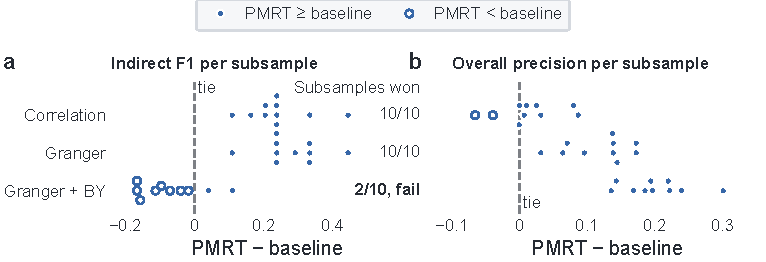
\includegraphics[width=\textwidth]{figures/fig_study1_subsamples.pdf}
\caption{Per-subsample comparison, randomised logs.}
\label{fig:s_subsamples}
\end{figure}

\FloatBarrier
\section{Conflict mitigation}
\label{esm:decision}

Tables~\ref{tab:s_arms} and~\ref{tab:s_arms2} give every arm of the two decision datasets, Figures~\ref{fig:s_deferrals} and~\ref{fig:s_cert} the rejected units and the certification per class, Table~\ref{tab:s_gate} the uncertified guard edges, and Tables~\ref{tab:s_x7} and~\ref{tab:s_blocks} the associational referees and the two seed blocks.

\begin{table}
\caption{All decision arms, without the gate.}
\label{tab:s_arms}
\footnotesize
\setlength{\tabcolsep}{2pt}
\begin{tabular}{@{}l c c c c c c c c c@{}}
\toprule
 & & & $\Delta R$ vs never-sleep & & \multicolumn{4}{c}{Guard ratio} & \\
\cmidrule(lr){6-9}
Arm & Rej. & $R$ & [90\,\% CI] & Ret. & SVR & eMBB & LL & RLF & Elig. \\
\midrule
\multicolumn{10}{@{}l}{\textbf{Without the gate}} \\
\multicolumn{10}{@{}l}{\textit{Static rules}} \\
\quad Accept-all & 0.00 & 0.00 & $-$0.22 [$-$0.30, $-$0.14] & 1.00 & 1.00 & 1.00 & 1.00 & 1.00 & yes \\
\quad Never-sleep & 0.06 & 0.22 & -- & 1.18 & 0.87 & 0.87 & 0.85 & 0.99 & yes \\
\quad Freeze & -- & $-$4.35 & -- & 0.00 & 0.58 & 0.49 & 0.27 & 0.94 & no \\
\quad Slice Guarantee only & -- & 1.00 & -- & $-$0.00 & 0.57 & 0.56 & 0.52 & 0.95 & no \\
\quad ES only & -- & $-$6.62 & -- & 0.52 & 0.76 & 0.65 & 0.32 & 1.02 & no \\
\quad Power ES only & -- & $-$7.50 & -- & 0.63 & 0.83 & 0.71 & 0.44 & 1.01 & no \\
\quad ES + Power ES only & -- & $-$10.02 & -- & 1.00 & 1.03 & 0.89 & 0.48 & 1.00 & yes \\
\quad Incumbent & -- & $-$0.07 & -- & 0.86 & 0.93 & 0.92 & 0.87 & 0.96 & no \\
\quad Static envelope & -- & 0.16 & -- & 1.44 & 1.00 & 1.00 & 1.10 & 1.16 & no \\
\midrule
\multicolumn{10}{@{}l}{\textit{Map-driven referees}} \\
\quad PMRT map & 0.37 & 0.47 & +0.25 [0.14, 0.36] & 1.67 & 0.86 & 0.86 & 0.94 & 1.31 & no \\
\quad Oracle map & 0.15 & 0.24 & +0.02 [$-$0.04, 0.09] & 1.32 & 0.88 & 0.88 & 0.88 & 1.01 & yes \\
\quad Random map & 0.50 & $-$0.42 & $-$0.64 [$-$0.78, $-$0.51] & 1.10 & 1.08 & 1.08 & 1.07 & 0.99 & yes \\
\quad No-map control & 0.16 & 0.23 & +0.01 [$-$0.08, 0.10] & 0.89 & 0.93 & 0.93 & 0.88 & 0.99 & no \\
\midrule
\multicolumn{10}{@{}l}{\textit{Referees on associational maps (tuned thresholds)}} \\
\quad Correlation & 0.01 & 0.03 & $-$0.19 [$-$0.26, $-$0.12] & 1.03 & 0.97 & 0.97 & 0.95 & 1.00 & yes \\
\quad Granger & 0.87 & $-$11.48 & $-$11.70 [$-$12.96, $-$10.63] & 1.44 & 1.16 & 0.99 & 0.65 & 1.18 & no \\
\quad SHAP-GBDT & 0.33 & $-$0.08 & $-$0.31 [$-$0.42, $-$0.18] & 1.44 & 1.12 & 1.11 & 1.27 & 1.19 & no \\
\quad INT$^{\mathrm{a}}$ & 0.00 & 0.00 & $-$0.22 [$-$0.30, $-$0.14] & 1.00 & 1.00 & 1.00 & 1.00 & 1.00 & yes \\
\quad QACM & 0.00 & 0.01 & $-$0.21 [$-$0.28, $-$0.13] & 0.99 & 1.00 & 1.00 & 1.00 & 1.00 & yes \\
\quad Two-tower & 0.86 & $-$10.25 & $-$10.47 [$-$11.63, $-$9.49] & 1.47 & 1.06 & 0.91 & 0.59 & 1.16 & no \\
\quad Granger + BY & 0.87 & $-$9.77 & $-$10.00 [$-$11.15, $-$9.03] & 1.52 & 1.02 & 0.87 & 0.56 & 1.27 & no \\
\midrule
\multicolumn{10}{@{}l}{\textit{Referees on associational maps (placebo-calibrated thresholds)}} \\
\quad Correlation$^{\mathrm{a}}$ & 0.00 & 0.00 & $-$0.22 [$-$0.30, $-$0.14] & 1.00 & 1.00 & 1.00 & 1.00 & 1.00 & yes \\
\quad Granger$^{\mathrm{a}}$ & 0.00 & 0.00 & $-$0.22 [$-$0.30, $-$0.14] & 1.00 & 1.00 & 1.00 & 1.00 & 1.00 & yes \\
\quad SHAP-GBDT & 0.87 & $-$9.68 & $-$9.90 [$-$11.05, $-$8.94] & 1.52 & 1.02 & 0.87 & 0.56 & 1.27 & no \\
\quad INT$^{\mathrm{a}}$ & 0.00 & 0.00 & $-$0.22 [$-$0.30, $-$0.14] & 1.00 & 1.00 & 1.00 & 1.00 & 1.00 & yes \\
\quad QACM & 0.00 & 0.01 & $-$0.21 [$-$0.28, $-$0.13] & 0.99 & 1.00 & 1.00 & 1.00 & 1.00 & yes \\
\quad Two-tower$^{\mathrm{a}}$ & 0.00 & 0.00 & $-$0.22 [$-$0.30, $-$0.14] & 1.00 & 1.00 & 1.00 & 1.00 & 1.00 & yes \\
\bottomrule
\end{tabular}

\par\smallskip
{\raggedright\footnotesize Rej., share of requests rejected; Ret., energy retention; SVR, service violations; eMBB, non-protected eMBB violations; LL, low-latency violations; Elig., eligible; --, not stored. $\Delta R$: arm minus never-sleep, 90~\% paired seed-bootstrap CI. $^{\mathrm{a}}$Same decisions as accept-all on every seed.\par}
\end{table}

\begin{table}
\caption{All decision arms, with the gate.}
\label{tab:s_arms2}
\footnotesize
\setlength{\tabcolsep}{2pt}
\begin{tabular}{@{}l c c c c c c c c c@{}}
\toprule
 & & & $\Delta R$ vs never-sleep & & \multicolumn{4}{c}{Guard ratio} & \\
\cmidrule(lr){6-9}
Arm & Rej. & $R$ & [90\,\% CI] & Ret. & SVR & eMBB & LL & RLF & Elig. \\
\midrule
\multicolumn{10}{@{}l}{\textbf{With the gate} (other seeds)} \\
\multicolumn{10}{@{}l}{\textit{Static rules}} \\
\quad Accept-all & 0.00 & 0.00 & $-$0.26 [$-$0.34, $-$0.17] & 1.00 & 1.00 & 1.00 & 1.00 & 1.00 & yes \\
\quad Never-sleep & 0.05 & 0.26 & -- & 1.15 & 0.88 & 0.88 & 0.86 & 0.96 & yes \\
\quad Freeze & -- & $-$5.09 & -- & 0.00 & 0.60 & 0.52 & 0.29 & 0.94 & no \\
\quad Slice Guarantee only & -- & 1.00 & -- & $-$0.00 & 0.60 & 0.59 & 0.54 & 0.95 & no \\
\quad ES only & -- & $-$7.11 & -- & 0.49 & 0.75 & 0.65 & 0.34 & 1.02 & no \\
\quad Power ES only & -- & $-$8.66 & -- & 0.64 & 0.86 & 0.74 & 0.46 & 0.95 & no \\
\quad ES + Power ES only & -- & $-$11.11 & -- & 1.00 & 1.03 & 0.89 & 0.51 & 0.99 & yes \\
\quad Incumbent & -- & $-$0.19 & -- & 0.86 & 0.95 & 0.95 & 0.92 & 0.94 & no \\
\midrule
\multicolumn{10}{@{}l}{\textit{Map-driven referees}} \\
\quad PMRT map & 0.05 & 0.26 & 0.00 [0.00, 0.00] & 1.15 & 0.88 & 0.88 & 0.86 & 0.96 & yes \\
\quad Ungated PMRT map & 0.352 & 0.20 & $-$0.06 [$-$0.22, 0.09] & 1.63 & 0.89 & 0.88 & 0.96 & 1.05 & yes \\
\quad Oracle map & 0.13 & 0.22 & $-$0.04 [$-$0.10, 0.03] & 1.29 & 0.90 & 0.90 & 0.91 & 0.94 & yes \\
\quad Random map$^{\mathrm{a}}$ & 0.00 & 0.00 & $-$0.26 [$-$0.34, $-$0.17] & 1.00 & 1.00 & 1.00 & 1.00 & 1.00 & yes \\
\quad No-map control$^{\mathrm{a}}$ & 0.00 & 0.00 & $-$0.26 [$-$0.34, $-$0.17] & 1.00 & 1.00 & 1.00 & 1.00 & 1.00 & yes \\
\midrule
\multicolumn{10}{@{}l}{\textit{Referees on associational maps (tuned thresholds)}} \\
\quad Correlation & 0.01 & 0.10 & $-$0.16 [$-$0.23, $-$0.10] & 1.03 & 0.97 & 0.97 & 0.97 & 0.97 & yes \\
\quad Granger & 0.80 & $-$11.06 & $-$11.31 [$-$12.97, $-$10.04] & 1.00 & 1.03 & 0.88 & 0.50 & 0.99 & yes \\
\quad SHAP-GBDT & 0.00 & $-$0.01 & $-$0.27 [$-$0.35, $-$0.18] & 1.00 & 1.00 & 1.00 & 1.00 & 1.00 & yes \\
\quad INT$^{\mathrm{a}}$ & 0.00 & 0.00 & $-$0.26 [$-$0.34, $-$0.17] & 1.00 & 1.00 & 1.00 & 1.00 & 1.00 & yes \\
\quad QACM$^{\mathrm{b}}$ & 0.00 & $-$0.01 & $-$0.27 [$-$0.35, $-$0.18] & 1.00 & 1.00 & 1.00 & 1.00 & 1.00 & yes \\
\quad Two-tower & 0.80 & $-$11.02 & $-$11.28 [$-$12.92, $-$10.01] & 1.00 & 1.03 & 0.88 & 0.50 & 0.99 & yes \\
\quad Granger + BY & 0.81 & $-$10.55 & $-$10.81 [$-$12.42, $-$9.55] & 1.03 & 1.00 & 0.86 & 0.49 & 0.97 & yes \\
\midrule
\multicolumn{10}{@{}l}{\textit{Referees on associational maps (placebo-calibrated thresholds)}} \\
\quad Correlation$^{\mathrm{a}}$ & 0.00 & 0.00 & $-$0.26 [$-$0.34, $-$0.17] & 1.00 & 1.00 & 1.00 & 1.00 & 1.00 & yes \\
\quad Granger$^{\mathrm{a}}$ & 0.00 & 0.00 & $-$0.26 [$-$0.34, $-$0.17] & 1.00 & 1.00 & 1.00 & 1.00 & 1.00 & yes \\
\quad SHAP-GBDT & 0.81 & $-$10.47 & $-$10.72 [$-$12.29, $-$9.49] & 1.03 & 1.00 & 0.86 & 0.50 & 0.97 & yes \\
\quad INT$^{\mathrm{a}}$ & 0.00 & 0.00 & $-$0.26 [$-$0.34, $-$0.17] & 1.00 & 1.00 & 1.00 & 1.00 & 1.00 & yes \\
\quad QACM$^{\mathrm{b}}$ & 0.00 & $-$0.01 & $-$0.27 [$-$0.35, $-$0.18] & 1.00 & 1.00 & 1.00 & 1.00 & 1.00 & yes \\
\quad Two-tower$^{\mathrm{a}}$ & 0.00 & 0.00 & $-$0.26 [$-$0.34, $-$0.17] & 1.00 & 1.00 & 1.00 & 1.00 & 1.00 & yes \\
\midrule
\multicolumn{10}{@{}l}{\textit{Random rejection}} \\
\quad $p = 0.25$ & 0.25 & $-$0.22 & $-$0.47 [$-$0.61, $-$0.35] & 1.02 & 0.99 & 0.99 & 0.94 & 0.99 & yes \\
\quad $p = 0.352$ & 0.35 & $-$0.46 & $-$0.71 [$-$0.87, $-$0.57] & 1.01 & 1.00 & 0.99 & 0.96 & 0.98 & yes \\
\quad $p = 0.50$ & 0.50 & $-$0.65 & $-$0.90 [$-$1.10, $-$0.73] & 1.03 & 0.99 & 0.98 & 0.91 & 0.95 & yes \\
\bottomrule
\end{tabular}

\par\smallskip
{\raggedright\footnotesize Rej., share of requests rejected; Ret., energy retention; SVR, service violations; eMBB, non-protected eMBB violations; LL, low-latency violations; Elig., eligible; --, not stored. $\Delta R$: arm minus never-sleep, 90~\% paired seed-bootstrap CI. $^{\mathrm{a}}$Same decisions as accept-all on every seed. Random rejection at $p = 0.352$ matches the ungated referee's rejection share, 37\,890 of 107\,525 requests. $^{\mathrm{b}}$After the gate, this map gives the referee the same decision rule as the SHAP-GBDT tuned-threshold map; the row repeats that map's simulation.\par}
\end{table}

\begin{figure}
\centering
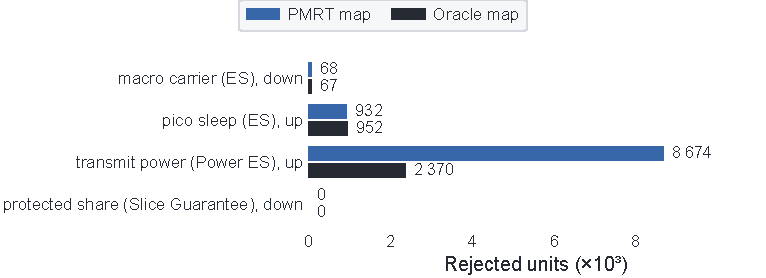
\includegraphics[width=\textwidth]{figures/fig_study2_deferrals.pdf}
\caption{Rejected units per class, referee without the gate.}
\label{fig:s_deferrals}
\end{figure}

\begin{figure}
\centering
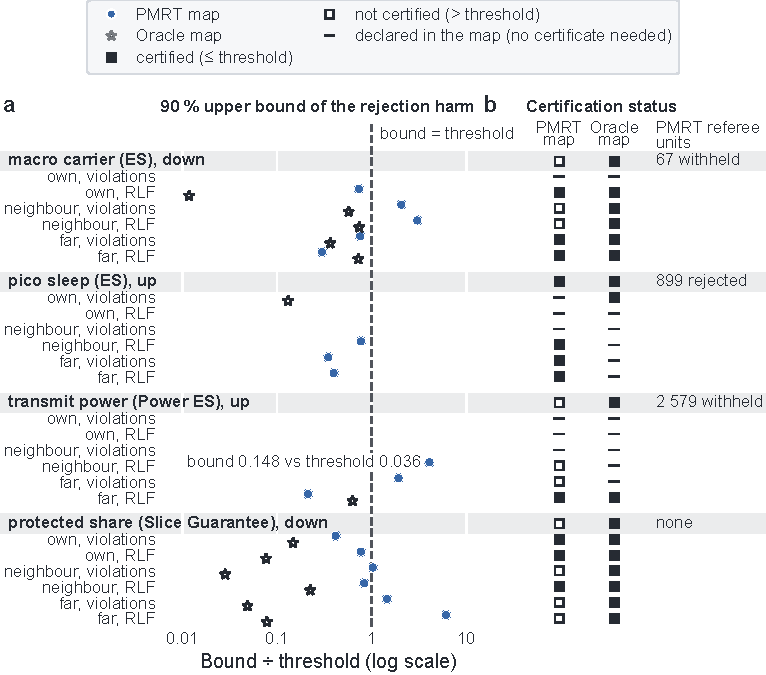
\includegraphics[width=\textwidth]{figures/fig_study3_certification.pdf}
\caption{Certification per class and guard edge, referee with the gate.}
\label{fig:s_cert}
\end{figure}

\begin{table}[tbp]
\caption{Gate diagnosis.}
\label{tab:s_gate}
% tab_gate_diag: generated by oran-causal-figures (packages/figures/src/oran_causal/figures/figs/tab_gate_diag.py); do not edit.
% Sources: data/records/posthoc_x9_x16/revision/x10_gate_diag.json, data/records/shap_rerun/overlay/system_artifacts/report_2026-10-02/figures_data.json
% Post hoc analysis X10: descriptive, no verdict; Study 3 unchanged.
% h = -d (harm of a rejection); UB90 = h x beta + 1.28 SE (PMRT design slope); an edge is certified iff UB90 <= tau.
% GT: Study 2 knockout ground truth (40 episodes, 95 % episode-cluster CI), harm of a rejection = h x GT mean.
% Units: Study 3 evaluation, 160 seeds; withheld = rejections the referee did not make (class uncertified).
% Needs \usepackage{booktabs}.
\footnotesize
\setlength{\tabcolsep}{3pt}
\begin{tabular}{@{}l r r r r l c@{}}
\toprule
 & \multicolumn{3}{c}{PMRT bound} & \multicolumn{3}{c}{Ground truth} \\
\cmidrule(lr){2-4}\cmidrule(lr){5-7}
Uncertified guard edge & $h\beta$ & UB90 & $\varepsilon$ & $h\cdot$GT [95\,\% CI] & Label & Harm $>\varepsilon$ \\
\midrule
\multicolumn{7}{@{}l}{\textit{Transmit power up (Power ES): uncertified; 2\,579 units withheld}} \\
\quad neighbour RLFs & 0.0825 & 0.148 & 0.0364 & 0.0611 [0.0271, 0.0962] & true & yes \\
\quad far violations & 21.2 & 39.8 & 20.8 & 24.2 [18.9, 29.9] & true & yes \\
\midrule
\multicolumn{7}{@{}l}{\textit{Pico sleep (ES): certified; 899 units rejected}} \\
\quad none & \multicolumn{6}{l}{--} \\
\midrule
\multicolumn{7}{@{}l}{\textit{Macro carrier off (ES): uncertified; 67 units withheld}} \\
\quad neighbour violations & 16.2 & 34.9 & 17.0 & 6.65 [4.19, 9.70] & null & no \\
\quad neighbour RLFs & 0.0267 & 0.0903 & 0.0298 & 0.00798 [$-$0.00532, 0.0220] & indet. & no \\
\midrule
\multicolumn{7}{@{}l}{\textit{Protected share down (Slice Guarantee): uncertified; 0 units withheld}} \\
\quad neighbour violations & $-$0.110 & 8.76 & 8.52 & 0.0125 [$-$0.216, 0.242] & null & no \\
\quad far violations & 4.16 & 12.4 & 8.52 & 0.0919 [$-$0.194, 0.416] & null & no \\
\quad far RLFs & 0.0599 & 0.0914 & 0.0150 & 0.000368 [0, 0.00117] & null & no \\
\bottomrule
\end{tabular}


\par\smallskip
{\raggedright\footnotesize
$h\beta$, PMRT's estimated harm; UB90, its upper 90~\% bound; $\varepsilon$, the tolerance; $h\cdot$GT, the
ground-truth harm; indet., indeterminate. With a strict outcome centre, which uses only units whose window had closed before the unit opened, all 22 map slopes kept their sign, with relative changes of $-2.9$ to $+6.5$~\%; the gate bounds moved by a median of \val{x16.gate.median_pct}~\% of their tolerance, and no class changed certification status.\par}
\end{table}

\begin{table}
\caption{Gated associational referees and the static ES + Power ES subset.}
\label{tab:s_x7}
% tab_appC_x7: generated by oran-causal-figures (packages/figures/src/oran_causal/figures/figs/tab_appC_x7.py); do not edit.
% Sources: data/records/shap_rerun/overlay/posthoc_x7/x7/x7_tables.json
% Post hoc check X7: descriptive, no hypothesis, no criterion, no verdict; Study 3 unchanged.
% 160 Study 3 evaluation seeds. (a) share of scored-window requests (t >= 120 s) on which the referee's accept / reject decision equals the subset's; subset stream = the subset applied, the referee queried in shadow (primary); own stream = the referee applied, the subset in shadow.
% (b) R and paired differences with 90 % paired seed-bootstrap CIs; dR = arm minus the subset; referee rows compare stored records, replay rows compare with the subset's re-run on the replay host (never mixing hosts). Identical seeds = seeds whose record equals the subset's in every outcome field (of 160). Dagger = not eligible (retention < .90); every other row is eligible.
% Host note (PAPER_PLAN X7.5): re-runs vs stored records differ on some seeds by a few violations, dR within [-0.0004, +0.0003].
% Needs \usepackage{booktabs}.
\footnotesize
\setlength{\tabcolsep}{1.5pt}
\begin{tabular}{@{}l c c c c c c@{}}
\toprule
\multicolumn{7}{@{}l}{(a) Agreement with the static subset's decision, per request} \\
\midrule
 & \multicolumn{5}{c}{Subset's request stream} & Own stream \\
\cmidrule(lr){2-6}\cmidrule(lr){7-7}
Map & Prot. share up & Tx power & Carrier & Sleep & All & All \\
\midrule
Granger & 1.0000 & 1.0000 & 0.9989 & 1.0000 & 0.9999 & 0.9996 \\
Granger + BY & 1.0000 & 1.0000 & 0.9989 & 0.9742 & 0.9994 & 0.9950 \\
Two-tower & 0.9993 & 1.0000 & 0.9989 & 1.0000 & 0.9994 & 0.9991 \\
SHAP-GBDT (placebo-cal.) & 0.9993 & 1.0000 & 0.9989 & 0.9742 & 0.9989 & 0.9941 \\
\midrule
Requests & 99\,785 & 5\,459 & 6\,476 & 2\,097 & 113\,817 & \\
\bottomrule
\end{tabular}

\par\medskip

\setlength{\tabcolsep}{2.5pt}
\begin{tabular}{@{}>{\raggedright\arraybackslash}p{3.7cm} c c c c@{}}
\toprule
\multicolumn{5}{@{}l}{(b) Outcomes, attribution replays and paired differences vs the static subset} \\
\midrule
 & & & $\Delta R$ vs subset & Identical \\
Arm & $R$ [90\,\% CI] & Retention & [90\,\% CI] & seeds \\
\midrule
Static subset & $-$11.106 [$-$12.779, $-$9.815] & 1.000 &  &  \\
Accept-all & 0.000 [0.000, 0.000] & 0.995 &  &  \\
\midrule
\multicolumn{5}{@{}l}{\textit{Gated referee, Granger map}} \\
\quad Referee & $-$11.057 [$-$12.726, $-$9.780] & 1.003 & +0.049 [$-$0.016, 0.127] & 117 \\
\quad Replay: protected-share rejections only & $-$11.106 [$-$12.779, $-$9.815] & 1.000 & 0.000 [0.000, 0.000] & 160 \\
\quad Replay: without it & $-$0.009 [$-$0.049, 0.024] & 0.996 & +11.096 [9.807, 12.762] & 0 \\
\midrule
\multicolumn{5}{@{}l}{\textit{Gated referee, Granger + BY map}} \\
\quad Referee & $-$10.551 [$-$12.176, $-$9.286] & 1.032 & +0.555 [0.389, 0.740] & 65 \\
\quad Replay: protected-share rejections only & $-$11.102 [$-$12.773, $-$9.814] & 1.000 & +0.004 [0.000, 0.012] & 159 \\
\quad Replay: without it & +0.071 [0.012, 0.133] & 1.028 & +11.177 [9.894, 12.844] & 0 \\
\midrule
\multicolumn{5}{@{}l}{\textit{Gated referee, Two-tower map}} \\
\quad Referee & $-$11.023 [$-$12.683, $-$9.745] & 1.003 & +0.083 [0.011, 0.166] & 109 \\
\quad Replay: protected-share rejections only & $-$11.072 [$-$12.735, $-$9.786] & 1.000 & +0.034 [0.007, 0.069] & 151 \\
\quad Replay: without it & $-$0.009 [$-$0.049, 0.024] & 0.996 & +11.096 [9.807, 12.762] & 0 \\
\midrule
\multicolumn{5}{@{}l}{\textit{Gated referee, SHAP-GBDT map, placebo-calibrated threshold}} \\
\quad Referee & $-$10.467 [$-$12.055, $-$9.215] & 1.033 & +0.639 [0.457, 0.848] & 33 \\
\quad Replay: protected-share rejections only & $-$11.072 [$-$12.735, $-$9.786] & 1.000 & +0.034 [0.007, 0.069] & 151 \\
\quad Replay: without it & +0.071 [0.012, 0.133] & 1.028 & +11.177 [9.894, 12.844] & 0 \\
\bottomrule
\end{tabular}


\par\smallskip
{\raggedright\footnotesize Identical seeds: seeds on which the arm equals the static subset.\par}
\end{table}

\begin{table}
\caption{Ungated PMRT referee on the two seed blocks.}
\label{tab:s_blocks}
\footnotesize
\setlength{\tabcolsep}{4pt}
\begin{tabular*}{\textwidth}{@{\extracolsep{\fill}}>{\raggedright}p{0.5\textwidth} c c@{}}
\toprule
 & Block without the gate & Block with the gate \\
\midrule
Contrast of never-sleep with accept-all & \val{x15.r.never_sleep_s2} & \val{x15.r.never_sleep_s3} \\
Share of requests rejected & \val{x15.rej.s2} & \val{x15.rej.s3} \\
Standard deviation of the per-seed difference from never-sleep & \val{x15.sd.s2} & \val{x15.sd.s3} \\
Estimate without the five seeds of largest contribution & $+\val{x15.trim.s2}$ & $+\val{x15.trim.s3}$ \\
\bottomrule
\end{tabular*}

\par\smallskip
{\raggedright\footnotesize Permutation test of the per-seed violation rate between blocks: $p = \val{x15.p.noarb}$ under accept-all, $p = \val{x15.p.never_sleep}$ under never-sleep. Difference of the block means: \val{x15.block_diff} (permutation $p = \val{x15.perm_p}$).\par}
\end{table}

\FloatBarrier
\section{Controlled environments}
\label{esm:envs}

Table~\ref{tab:s_claims} counts conditions by group of tests and Table~\ref{tab:s_verdicts} by environment, with rates and conditions classed as invalid, valid or inconclusive by the rule of Section~5.4 of the article. Figure~\ref{fig:s_validity_env} shows the null-edge rate by environment, Tables~\ref{tab:s_env1} to~\ref{tab:s_env5} the null-edge rate and recall per environment, Figure~\ref{fig:s_recall} the recall against sample size, and Tables~\ref{tab:s_dose} and~\ref{tab:s_misspec} the null rates under other dither designs and under a misspecified design. Both PMRT variants here omit the Huber clip of the unit weight.

\begin{table}
\caption{Conditions by group of tests under the controlled environments.}
\label{tab:s_claims}
\footnotesize
\setlength{\tabcolsep}{3pt}
\begin{tabular*}{\textwidth}{@{\extracolsep{\fill}}p{3.7cm} p{2.6cm} c p{2.6cm}@{}}
\toprule
Group and design & Methods & \shortstack{Invalid / valid\\/ counted} & Pooled rate \tabularnewline
\midrule
\raggedright Design-blind, dithered setpoint & \raggedright Six design-blind tests & 95 / 7 / 115 & \raggedright 0.33 to 0.94 (truth-null) \tabularnewline
\raggedright Design-based, independent and dithered & \raggedright PMRT-GBM & 1 / 18 / 50 & \raggedright truth-null 0.045 (0.043--0.048); placebo 0.048 (0.042--0.054) \tabularnewline
\raggedright Design-adjusted, independent and dithered & \raggedright Partial correlation, Granger & 0 / 21 / 60 & \raggedright 0.048 and 0.051; 0.050 and 0.056 \tabularnewline
\raggedright Design-based, confounded policy & \raggedright PMRT-GBM & 0 / 6 / 20 & \raggedright confounded null 0.042; placebo 0.048 \tabularnewline
\bottomrule
\end{tabular*}

\par\medskip

\begin{tabular*}{\textwidth}{@{\extracolsep{\fill}}l c c l c c@{}}
\toprule
\multicolumn{6}{@{}l}{Design-blind tests under dithered logging: pooled truth-null rate and invalid / planned conditions} \tabularnewline
\midrule
Correlation & 0.79 & 22 / 25 & Partial correlation, HAC fixed-bandwidth & 0.47 & 20 / 25 \tabularnewline
Plain Granger & 0.69 & 5 / 5 & Plain RCoT & 0.33 & 20 / 25 \tabularnewline
Plain partial correlation & 0.47 & 20 / 25 & MSCR & 0.94 & 8 / 10 \tabularnewline
\bottomrule
\end{tabular*}
\end{table}

\begin{table}
\caption{Conditions by environment.}
\label{tab:s_verdicts}
\footnotesize
\setlength{\tabcolsep}{2pt}
\begin{tabular}{@{}l c c c c c c@{}}
\toprule
\multicolumn{7}{@{}l}{Invalid / valid / counted over every $n$ at $\kappa = 0.25$; the remainder are inconclusive} \\
\midrule
Group and design & Linear & Rare & Delayed & Confounding & Composed & All \\
\midrule
Design-blind, dithered & 22/0/22 & 22/0/22 & 27/0/27 & 2/7/22 & 22/0/22 & 95/7/115 \\
Design-based, independent and dithered & 1/0/10 & 0/7/10 & 0/3/10 & 0/5/10 & 0/3/10 & 1/18/50 \\
Design-adjusted, independent and dithered & 0/3/10 & 0/6/10 & 0/4/20 & 0/5/10 & 0/3/10 & 0/21/60 \\
Design-based, confounded policy & -- & -- & -- & 0/6/20 & -- & 0/6/20 \\
\bottomrule
\end{tabular}

\end{table}

Tables~\ref{tab:s_env1} to~\ref{tab:s_env5} give every condition at the primary observation noise $\kappa = 0.25$ with 40 seeds per condition. Each cell gives the null-edge rate and the recall: the rate is the share of truth-null edges with $p \le 0.05$, or the share declared for the methods that use a threshold, and recall is read under BY or the threshold. An asterisk marks an invalid condition, whose recall is not reported, a tilde an inconclusive condition and a circle a condition with no validity read; in the latent-confounding environment the rate is that of the placebo edge at $\lambda = 1$.

\begin{figure}
\centering
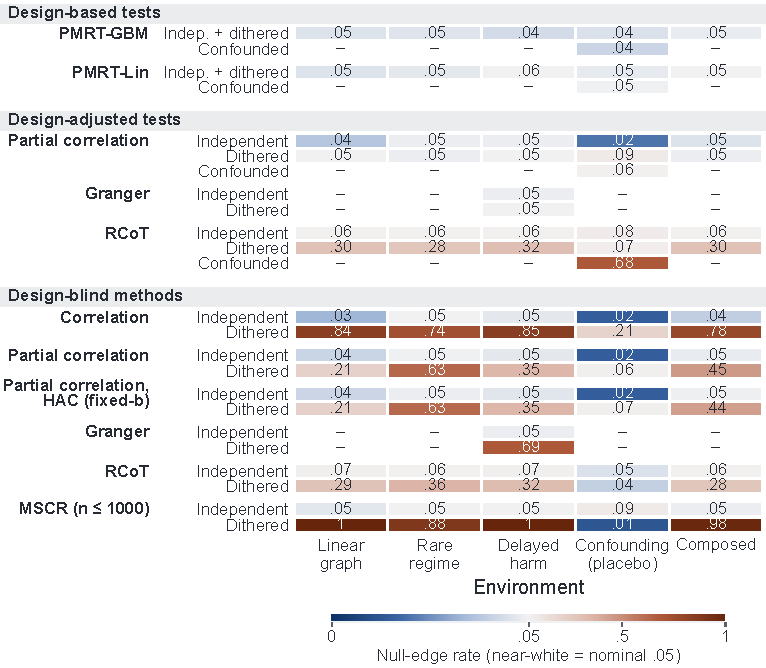
\includegraphics[width=\textwidth]{figures/fig_study4_validity_env.pdf}
\caption{Null-edge rate by environment.}
\label{fig:s_validity_env}
\end{figure}

\begin{table}
\caption{Linear graph: null-edge rate / recall.}
\label{tab:s_env1}
% tab_study4_env_e1: generated by oran-causal-figures (packages/figures/src/oran_causal/figures/figs/tab_study4_env.py); do not edit.
% Sources: data/records/study4_eval/eval/csv/validity_cells.csv, data/records/study4_eval/eval/csv/recall_vs_n.csv
% Entry: null-edge rejection rate / recall; mark = the condition's validity from all its reads (* INVALID, ~ INCONCLUSIVE, unmarked VALID, ° no validity read); -- = no recall (INVALID condition); blank = not in the method's grid. Needs \usepackage{booktabs}.
\setlength{\tabcolsep}{2.8pt}
\begin{tabular}{@{}l c c c c c@{}}
\toprule
Method & $n=500$ & $n=1000$ & $n=4000$ & $n=8000$ & $n=24000$ \\
\midrule
\multicolumn{6}{@{}l}{\textbf{E1, R1}} \\
\multicolumn{6}{@{}l}{\textit{Design-based tests}} \\
\quad PMRT-GBM & 0.027$^{\textstyle\sim}$/1.00 & 0.033$^{\textstyle\sim}$/1.00 & 0.044$^{\textstyle\sim}$/1.00 & 0.050$^{\textstyle\sim}$/1.00 & 0.056$^{\textstyle\sim}$/1.00 \\
\quad PMRT-Lin & 0.037/1.00 & 0.033$^{\textstyle\sim}$/1.00 & 0.052$^{\textstyle\sim}$/1.00 & 0.037$^{\textstyle\sim}$/1.00 & 0.044$^{\textstyle\sim}$/1.00 \\
\multicolumn{6}{@{}l}{\textit{Design-adjusted tests}} \\
\quad Partial correlation & 0.029/1.00 & 0.025/1.00 & 0.046$^{\textstyle\sim}$/1.00 & 0.037$^{\textstyle\sim}$/1.00 & 0.050$^{\textstyle\sim}$/1.00 \\
\quad RCoT & 0.083$^{\textstyle *}$/-- & 0.069$^{\textstyle\sim}$/1.00 & 0.060$^{\textstyle\sim}$/1.00 & 0.050$^{\textstyle\sim}$/1.00 & 0.046$^{\textstyle\sim}$/1.00 \\
\multicolumn{6}{@{}l}{\textit{Design-blind methods}} \\
\quad Correlation & 0.037/1.00 & 0.019/1.00 & 0.056$^{\textstyle\sim}$/1.00 & 0.029$^{\textstyle\sim}$/1.00 & 0.023$^{\textstyle\sim}$/1.00 \\
\quad Partial correlation & 0.040/1.00 & 0.033/1.00 & 0.050$^{\textstyle\sim}$/1.00 & 0.046$^{\textstyle\sim}$/1.00 & 0.037$^{\textstyle\sim}$/1.00 \\
\quad Partial correlation, HAC & 0.044$^{\textstyle\sim}$/1.00 & 0.035/1.00 & 0.048$^{\textstyle\sim}$/1.00 & 0.044$^{\textstyle\sim}$/1.00 & 0.037$^{\textstyle\sim}$/1.00 \\
\quad Partial correlation, HAC (fixed-b) & 0.044$^{\textstyle\sim}$/1.00 & 0.035/1.00 & 0.048$^{\textstyle\sim}$/1.00 & 0.044$^{\textstyle\sim}$/1.00 & 0.037$^{\textstyle\sim}$/1.00 \\
\quad RCoT & 0.094$^{\textstyle *}$/-- & 0.094$^{\textstyle *}$/-- & 0.062$^{\textstyle\sim}$/1.00 & 0.060$^{\textstyle\sim}$/1.00 & 0.035$^{\textstyle\sim}$/1.00 \\
\quad MSCR (n $\le$ 1000) & 0.040$^{\textstyle\sim}$/1.00 & 0.054/1.00 &  &  &  \\
\quad PC & 0.094$^{\textstyle *}$/-- & 0.025/1.00 & 0.042/1.00 & 0.019/1.00 & 0.054$^{\textstyle\sim}$/1.00 \\
\quad NOTEARS & 0.000/1.00 & 0.000/1.00 & 0.000/1.00 & 0.000/1.00 & 0.000/1.00 \\
\quad SHAP-DAG & 0.035/1.00 & 0.029/1.00 & 0.133$^{\textstyle *}$/-- & 0.125$^{\textstyle *}$/-- & 0.037/1.00 \\
\quad Two-tower & 0.021/1.00 & 0.025/1.00 & 0.027/1.00 & 0.033/1.00 & 0.044/1.00 \\
\quad CDD O-RAN discovery & 0.075$^{\textstyle *}$/-- & 0.081$^{\textstyle *}$/-- & 0.037/1.00 &  &  \\
\midrule
\multicolumn{6}{@{}l}{\textbf{E1, R2}} \\
\multicolumn{6}{@{}l}{\textit{Design-based tests}} \\
\quad PMRT-GBM & 0.033$^{\textstyle\sim}$/1.00 & 0.033$^{\textstyle\sim}$/1.00 & 0.040$^{\textstyle\sim}$/1.00 & 0.062$^{\textstyle\sim}$/1.00 & 0.075$^{\textstyle *}$/-- \\
\quad PMRT-Lin & 0.048$^{\textstyle\sim}$/0.96 & 0.050/0.97 & 0.054$^{\textstyle\sim}$/0.99 & 0.050/0.99 & 0.048$^{\textstyle\sim}$/0.99 \\
\multicolumn{6}{@{}l}{\textit{Design-adjusted tests}} \\
\quad Partial correlation & 0.056$^{\textstyle\sim}$/1.00 & 0.042$^{\textstyle\sim}$/1.00 & 0.054$^{\textstyle\sim}$/1.00 & 0.056$^{\textstyle\sim}$/1.00 & 0.042/1.00 \\
\quad RCoT & 0.104$^{\textstyle *}$/-- & 0.083$^{\textstyle *}$/-- & 0.237$^{\textstyle *}$/-- & 0.369$^{\textstyle *}$/-- & 0.708$^{\textstyle *}$/-- \\
\multicolumn{6}{@{}l}{\textit{Design-blind methods}} \\
\quad Correlation & 0.683$^{\textstyle *}$/-- & 0.758$^{\textstyle *}$/-- & 0.887$^{\textstyle *}$/-- & 0.921$^{\textstyle *}$/-- & 0.954$^{\textstyle *}$/-- \\
\quad Partial correlation & 0.210$^{\textstyle *}$/-- & 0.198$^{\textstyle *}$/-- & 0.198$^{\textstyle *}$/-- & 0.225$^{\textstyle *}$/-- & 0.242$^{\textstyle *}$/-- \\
\quad Partial correlation, HAC & 0.212$^{\textstyle *}$/-- & 0.198$^{\textstyle *}$/-- & 0.196$^{\textstyle *}$/-- & 0.225$^{\textstyle *}$/-- & 0.242$^{\textstyle *}$/-- \\
\quad Partial correlation, HAC (fixed-b) & 0.210$^{\textstyle *}$/-- & 0.198$^{\textstyle *}$/-- & 0.196$^{\textstyle *}$/-- & 0.225$^{\textstyle *}$/-- & 0.242$^{\textstyle *}$/-- \\
\quad RCoT & 0.156$^{\textstyle *}$/-- & 0.152$^{\textstyle *}$/-- & 0.204$^{\textstyle *}$/-- & 0.344$^{\textstyle *}$/-- & 0.610$^{\textstyle *}$/-- \\
\quad MSCR (n $\le$ 1000) & 1.000$^{\textstyle *}$/-- & 1.000$^{\textstyle *}$/-- &  &  &  \\
\quad PC & 0.067$^{\textstyle\sim}$/1.00 & 0.027/1.00 & 0.027/1.00 & 0.065$^{\textstyle\sim}$/1.00 & 0.048/1.00 \\
\quad NOTEARS & 0.165$^{\textstyle *}$/-- & 0.169$^{\textstyle *}$/-- & 0.167$^{\textstyle *}$/-- & 0.169$^{\textstyle *}$/-- & 0.169$^{\textstyle *}$/-- \\
\quad SHAP-DAG & 0.246$^{\textstyle *}$/-- & 0.225$^{\textstyle *}$/-- & 0.219$^{\textstyle *}$/-- & 0.202$^{\textstyle *}$/-- & 0.198$^{\textstyle *}$/-- \\
\quad Two-tower & 0.198$^{\textstyle *}$/-- & 0.204$^{\textstyle *}$/-- & 0.212$^{\textstyle *}$/-- & 0.196$^{\textstyle *}$/-- & 0.223$^{\textstyle *}$/-- \\
\quad CDD O-RAN discovery & 0.027/1.00 & 0.106$^{\textstyle *}$/-- & 0.183$^{\textstyle *}$/-- &  &  \\
\bottomrule
\end{tabular}

\end{table}

\begin{table}
\caption{Rare regime: null-edge rate / recall.}
\label{tab:s_env2}
% tab_study4_env_e2: generated by oran-causal-figures (packages/figures/src/oran_causal/figures/figs/tab_study4_env.py); do not edit.
% Sources: data/records/study4_eval/eval/csv/validity_cells.csv, data/records/study4_eval/eval/csv/recall_vs_n.csv
% Entry: null-edge rejection rate / recall; mark = the condition's validity from all its reads (* INVALID, ~ INCONCLUSIVE, unmarked VALID, ° no validity read); -- = no recall (INVALID condition); blank = not in the method's grid. Needs \usepackage{booktabs}.
\footnotesize
\setlength{\tabcolsep}{2.5pt}
\begin{tabular}{@{}>{\raggedright\arraybackslash}p{3.3cm} c c c c c@{}}
\toprule
Method & $n=500$ & $n=1000$ & $n=4000$ & $n=8000$ & $n=24000$ \\
\midrule
\multicolumn{6}{@{}l}{\textbf{Rare regime, independent logging}} \\
\multicolumn{6}{@{}l}{\textit{Design-based tests}} \\
\quad PMRT-GBM & 0.041/0.79 & 0.037/0.83 & 0.045/0.94 & 0.045/0.95 & 0.045$^{\textstyle\sim}$/0.99 \\
\quad PMRT-Lin & 0.051$^{\textstyle\sim}$/0.29 & 0.046/0.32 & 0.050$^{\textstyle\sim}$/0.34 & 0.035/0.37 & 0.050$^{\textstyle\sim}$/0.38 \\
\multicolumn{6}{@{}l}{\textit{Design-adjusted tests}} \\
\quad Partial correlation & 0.054$^{\textstyle\sim}$/0.28 & 0.047/0.32 & 0.054/0.34 & 0.038/0.37 & 0.050$^{\textstyle\sim}$/0.38 \\
\quad RCoT & 0.094$^{\textstyle *}$/-- & 0.065$^{\textstyle *}$/-- & 0.052$^{\textstyle\sim}$/0.60 & 0.051/0.62 & 0.041/0.67 \\
\multicolumn{6}{@{}l}{\textit{Design-blind methods}} \\
\quad Correlation & 0.055$^{\textstyle\sim}$/0.30 & 0.052/0.32 & 0.053/0.35 & 0.040$^{\textstyle\sim}$/0.36 & 0.053$^{\textstyle\sim}$/0.38 \\
\quad Partial correlation & 0.060$^{\textstyle\sim}$/0.29 & 0.046$^{\textstyle\sim}$/0.32 & 0.052/0.34 & 0.038/0.36 & 0.052$^{\textstyle\sim}$/0.38 \\
\quad Partial correlation, HAC & 0.055$^{\textstyle\sim}$/0.31 & 0.045$^{\textstyle\sim}$/0.31 & 0.052/0.34 & 0.040/0.36 & 0.052$^{\textstyle\sim}$/0.38 \\
\quad Partial correlation, HAC (fixed-b) & 0.055$^{\textstyle\sim}$/0.31 & 0.044$^{\textstyle\sim}$/0.31 & 0.052/0.34 & 0.040/0.36 & 0.052$^{\textstyle\sim}$/0.38 \\
\quad RCoT & 0.097$^{\textstyle *}$/-- & 0.059$^{\textstyle\sim}$/0.56 & 0.052/0.60 & 0.051/0.62 & 0.046/0.67 \\
\quad MSCR (n $\le$ 1000) & 0.054/0.88 & 0.046/0.94 &  &  &  \\
\quad PC & 0.069$^{\textstyle *}$/-- & 0.065$^{\textstyle *}$/-- & 0.022/0.38 & 0.012/0.38 & 0.055/0.41 \\
\quad NOTEARS & 0.016/0.25 & 0.000/0.26 & 0.000/0.25 & 0.000/0.25 & 0.000/0.25 \\
\quad SHAP-DAG & 0.065$^{\textstyle *}$/-- & 0.041/0.95 & 0.041/0.99 & 0.056/1.00 & 0.032/1.00 \\
\quad Two-tower & 0.083$^{\textstyle *}$/-- & 0.041/0.67 & 0.051/0.78 & 0.081$^{\textstyle *}$/-- & 0.176$^{\textstyle *}$/-- \\
\quad CDD O-RAN discovery & 0.073$^{\textstyle *}$/-- & 0.078$^{\textstyle *}$/-- & 0.050/0.96 &  &  \\
\midrule
\multicolumn{6}{@{}l}{\textbf{Rare regime, dithered setpoint}} \\
\multicolumn{6}{@{}l}{\textit{Design-based tests}} \\
\quad PMRT-GBM & 0.052/0.49 & 0.049$^{\textstyle\sim}$/0.66 & 0.052/0.93 & 0.041$^{\textstyle\sim}$/0.93 & 0.051/0.94 \\
\quad PMRT-Lin & 0.057/0.19 & 0.053/0.28 & 0.037/0.45 & 0.034/0.55 & 0.058/0.68 \\
\multicolumn{6}{@{}l}{\textit{Design-adjusted tests}} \\
\quad Partial correlation & 0.055$^{\textstyle\sim}$/0.30 & 0.059/0.37 & 0.039/0.54 & 0.035$^{\textstyle\sim}$/0.63 & 0.055/0.76 \\
\quad RCoT & 0.135$^{\textstyle *}$/-- & 0.112$^{\textstyle *}$/-- & 0.227$^{\textstyle *}$/-- & 0.355$^{\textstyle *}$/-- & 0.552$^{\textstyle *}$/-- \\
\multicolumn{6}{@{}l}{\textit{Design-blind methods}} \\
\quad Correlation & 0.506$^{\textstyle *}$/-- & 0.606$^{\textstyle *}$/-- & 0.795$^{\textstyle *}$/-- & 0.858$^{\textstyle *}$/-- & 0.918$^{\textstyle *}$/-- \\
\quad Partial correlation & 0.352$^{\textstyle *}$/-- & 0.468$^{\textstyle *}$/-- & 0.691$^{\textstyle *}$/-- & 0.784$^{\textstyle *}$/-- & 0.873$^{\textstyle *}$/-- \\
\quad Partial correlation, HAC & 0.341$^{\textstyle *}$/-- & 0.471$^{\textstyle *}$/-- & 0.691$^{\textstyle *}$/-- & 0.780$^{\textstyle *}$/-- & 0.862$^{\textstyle *}$/-- \\
\quad Partial correlation, HAC (fixed-b) & 0.340$^{\textstyle *}$/-- & 0.470$^{\textstyle *}$/-- & 0.690$^{\textstyle *}$/-- & 0.779$^{\textstyle *}$/-- & 0.862$^{\textstyle *}$/-- \\
\quad RCoT & 0.167$^{\textstyle *}$/-- & 0.189$^{\textstyle *}$/-- & 0.304$^{\textstyle *}$/-- & 0.454$^{\textstyle *}$/-- & 0.674$^{\textstyle *}$/-- \\
\quad MSCR (n $\le$ 1000) & 0.841$^{\textstyle *}$/-- & 0.924$^{\textstyle *}$/-- &  &  &  \\
\quad PC & 0.023/0.24 & 0.035/0.29 & 0.021/0.26 & 0.000/0.00 & 0.000/0.00 \\
\quad NOTEARS & 0.033/0.28 & 0.037/0.29 & 0.041/0.30 & 0.029/0.29 & 0.028/0.28 \\
\quad SHAP-DAG & 0.030/0.77 & 0.046/0.91 & 0.032/0.96 & 0.054/0.97 & 0.050/0.98 \\
\quad Two-tower & 0.062$^{\textstyle\sim}$/0.55 & 0.016/0.42 & 0.045/0.66 & 0.028/0.58 & 0.028/0.60 \\
\quad CDD O-RAN discovery & 0.030/0.40 & 0.027/0.49 & 0.037/0.80 &  &  \\
\bottomrule
\end{tabular}

\end{table}

\begin{table}
\caption{Delayed harm: null-edge rate / recall.}
\label{tab:s_env3}
% tab_study4_env_e3: generated by oran-causal-figures (packages/figures/src/oran_causal/figures/figs/tab_study4_env.py); do not edit.
% Sources: data/records/study4_eval/eval/csv/validity_cells.csv, data/records/study4_eval/eval/csv/recall_vs_n.csv
% Entry: null-edge rejection rate / recall; mark = the condition's validity from all its reads (* INVALID, ~ INCONCLUSIVE, unmarked VALID, ° no validity read); -- = no recall (INVALID condition); blank = not in the method's grid. Needs \usepackage{booktabs}.
\setlength{\tabcolsep}{2.8pt}
\begin{tabular}{@{}l c c c c c@{}}
\toprule
Method & $n=500$ & $n=1000$ & $n=4000$ & $n=8000$ & $n=24000$ \\
\midrule
\multicolumn{6}{@{}l}{\textbf{E3, R1}} \\
\multicolumn{6}{@{}l}{\textit{Design-based tests}} \\
\quad PMRT-GBM & 0.036$^{\textstyle\sim}$/1.00 & 0.039$^{\textstyle\sim}$/1.00 & 0.042/1.00 & 0.048/1.00 & 0.034/1.00 \\
\quad PMRT-Lin & 0.037/1.00 & 0.059$^{\textstyle\sim}$/1.00 & 0.047$^{\textstyle\sim}$/1.00 & 0.045$^{\textstyle\sim}$/1.00 & 0.058/1.00 \\
\multicolumn{6}{@{}l}{\textit{Design-adjusted tests}} \\
\quad Partial correlation & 0.042$^{\textstyle\sim}$/1.00 & 0.050$^{\textstyle\sim}$/1.00 & 0.050$^{\textstyle\sim}$/1.00 & 0.045/1.00 & 0.055$^{\textstyle\sim}$/1.00 \\
\quad Granger & 0.042$^{\textstyle\sim}$/1.00 & 0.050$^{\textstyle\sim}$/1.00 & 0.050$^{\textstyle\sim}$/1.00 & 0.045/1.00 & 0.055$^{\textstyle\sim}$/1.00 \\
\quad RCoT & 0.098$^{\textstyle *}$/-- & 0.069$^{\textstyle\sim}$/1.00 & 0.055$^{\textstyle\sim}$/1.00 & 0.048$^{\textstyle\sim}$/1.00 & 0.045/1.00 \\
\multicolumn{6}{@{}l}{\textit{Design-blind methods}} \\
\quad Correlation & 0.044$^{\textstyle\sim}$/1.00 & 0.052/1.00 & 0.058$^{\textstyle\sim}$/1.00 & 0.027$^{\textstyle\sim}$/1.00 & 0.056$^{\textstyle\sim}$/1.00 \\
\quad Partial correlation & 0.037$^{\textstyle\sim}$/1.00 & 0.050$^{\textstyle\sim}$/1.00 & 0.048/1.00 & 0.042$^{\textstyle\sim}$/1.00 & 0.056$^{\textstyle\sim}$/1.00 \\
\quad Partial correlation, HAC & 0.037$^{\textstyle\sim}$/1.00 & 0.048$^{\textstyle\sim}$/1.00 & 0.048/1.00 & 0.042$^{\textstyle\sim}$/1.00 & 0.056$^{\textstyle\sim}$/1.00 \\
\quad Partial correlation, HAC (fixed-b) & 0.037$^{\textstyle\sim}$/1.00 & 0.048$^{\textstyle\sim}$/1.00 & 0.048/1.00 & 0.041$^{\textstyle\sim}$/1.00 & 0.056$^{\textstyle\sim}$/1.00 \\
\quad Granger & 0.045$^{\textstyle\sim}$/1.00 & 0.053/1.00 & 0.058$^{\textstyle\sim}$/1.00 & 0.030$^{\textstyle\sim}$/1.00 & 0.056$^{\textstyle\sim}$/1.00 \\
\quad RCoT & 0.084$^{\textstyle *}$/-- & 0.080$^{\textstyle *}$/-- & 0.053/1.00 & 0.047/1.00 & 0.061$^{\textstyle\sim}$/1.00 \\
\quad MSCR (n $\le$ 1000) & 0.044/1.00 & 0.056/1.00 &  &  &  \\
\quad PC & 0.017/1.00 & 0.045/1.00 & 0.045/1.00 & 0.064$^{\textstyle\sim}$/1.00 & 0.037/1.00 \\
\quad NOTEARS & 0.000/1.00 & 0.000/1.00 & 0.000/1.00 & 0.000/1.00 & 0.000/1.00 \\
\quad SHAP-DAG & 0.044/1.00 & 0.091$^{\textstyle *}$/-- & 0.048/1.00 & 0.103$^{\textstyle *}$/-- & 0.056/1.00 \\
\quad Two-tower & 0.072$^{\textstyle *}$/-- & 0.053/1.00 & 0.058/1.00 & 0.061/1.00 & 0.125$^{\textstyle *}$/-- \\
\quad CDD O-RAN discovery & 0.034/1.00 & 0.047/1.00 & 0.017/1.00 &  &  \\
\midrule
\multicolumn{6}{@{}l}{\textbf{E3, R2}} \\
\multicolumn{6}{@{}l}{\textit{Design-based tests}} \\
\quad PMRT-GBM & 0.034$^{\textstyle\sim}$/1.00 & 0.045$^{\textstyle\sim}$/1.00 & 0.048$^{\textstyle\sim}$/1.00 & 0.044$^{\textstyle\sim}$/1.00 & 0.058$^{\textstyle\sim}$/1.00 \\
\quad PMRT-Lin & 0.072$^{\textstyle\sim}$/0.98 & 0.062$^{\textstyle\sim}$/1.00 & 0.066$^{\textstyle\sim}$/1.00 & 0.064$^{\textstyle\sim}$/1.00 & 0.045/1.00 \\
\multicolumn{6}{@{}l}{\textit{Design-adjusted tests}} \\
\quad Partial correlation & 0.056$^{\textstyle\sim}$/1.00 & 0.052$^{\textstyle\sim}$/1.00 & 0.059$^{\textstyle\sim}$/1.00 & 0.056$^{\textstyle\sim}$/1.00 & 0.036/1.00 \\
\quad Granger & 0.056$^{\textstyle\sim}$/1.00 & 0.052$^{\textstyle\sim}$/1.00 & 0.059$^{\textstyle\sim}$/1.00 & 0.056$^{\textstyle\sim}$/1.00 & 0.036/1.00 \\
\quad RCoT & 0.111$^{\textstyle *}$/-- & 0.086$^{\textstyle *}$/-- & 0.253$^{\textstyle *}$/-- & 0.423$^{\textstyle *}$/-- & 0.706$^{\textstyle *}$/-- \\
\multicolumn{6}{@{}l}{\textit{Design-blind methods}} \\
\quad Correlation & 0.691$^{\textstyle *}$/-- & 0.784$^{\textstyle *}$/-- & 0.903$^{\textstyle *}$/-- & 0.920$^{\textstyle *}$/-- & 0.939$^{\textstyle *}$/-- \\
\quad Partial correlation & 0.216$^{\textstyle *}$/-- & 0.255$^{\textstyle *}$/-- & 0.366$^{\textstyle *}$/-- & 0.436$^{\textstyle *}$/-- & 0.480$^{\textstyle *}$/-- \\
\quad Partial correlation, HAC & 0.219$^{\textstyle *}$/-- & 0.255$^{\textstyle *}$/-- & 0.370$^{\textstyle *}$/-- & 0.442$^{\textstyle *}$/-- & 0.483$^{\textstyle *}$/-- \\
\quad Partial correlation, HAC (fixed-b) & 0.217$^{\textstyle *}$/-- & 0.255$^{\textstyle *}$/-- & 0.370$^{\textstyle *}$/-- & 0.442$^{\textstyle *}$/-- & 0.483$^{\textstyle *}$/-- \\
\quad Granger & 0.439$^{\textstyle *}$/-- & 0.558$^{\textstyle *}$/-- & 0.744$^{\textstyle *}$/-- & 0.798$^{\textstyle *}$/-- & 0.892$^{\textstyle *}$/-- \\
\quad RCoT & 0.159$^{\textstyle *}$/-- & 0.184$^{\textstyle *}$/-- & 0.248$^{\textstyle *}$/-- & 0.372$^{\textstyle *}$/-- & 0.647$^{\textstyle *}$/-- \\
\quad MSCR (n $\le$ 1000) & 1.000$^{\textstyle *}$/-- & 1.000$^{\textstyle *}$/-- &  &  &  \\
\quad PC & 0.130$^{\textstyle *}$/-- & 0.114$^{\textstyle *}$/-- & 0.128$^{\textstyle *}$/-- & 0.119$^{\textstyle *}$/-- & 0.158$^{\textstyle *}$/-- \\
\quad NOTEARS & 0.180$^{\textstyle *}$/-- & 0.189$^{\textstyle *}$/-- & 0.188$^{\textstyle *}$/-- & 0.188$^{\textstyle *}$/-- & 0.188$^{\textstyle *}$/-- \\
\quad SHAP-DAG & 0.250$^{\textstyle *}$/-- & 0.242$^{\textstyle *}$/-- & 0.228$^{\textstyle *}$/-- & 0.230$^{\textstyle *}$/-- & 0.230$^{\textstyle *}$/-- \\
\quad Two-tower & 0.222$^{\textstyle *}$/-- & 0.256$^{\textstyle *}$/-- & 0.242$^{\textstyle *}$/-- & 0.264$^{\textstyle *}$/-- & 0.255$^{\textstyle *}$/-- \\
\quad CDD O-RAN discovery & 0.111$^{\textstyle *}$/-- & 0.163$^{\textstyle *}$/-- & 0.205$^{\textstyle *}$/-- &  &  \\
\bottomrule
\end{tabular}

\end{table}

\begin{table}
\caption{Latent confounding: null-edge rate / recall.}
\label{tab:s_env4}
% tab_study4_env_e4: generated by oran-causal-figures (packages/figures/src/oran_causal/figures/figs/tab_study4_env.py); do not edit.
% Sources: data/records/study4_eval/eval/csv/validity_cells.csv, data/records/study4_eval/eval/csv/recall_vs_n.csv
% Entry: null-edge rejection rate / recall; mark = the condition's validity from all its reads (* INVALID, ~ INCONCLUSIVE, unmarked VALID, ° no validity read); -- = no recall (INVALID condition); blank = not in the method's grid. Needs \usepackage{booktabs}.
\setlength{\tabcolsep}{2.8pt}
\begin{tabular}{@{}l c c c c c@{}}
\toprule
Method & $n=500$ & $n=1000$ & $n=4000$ & $n=8000$ & $n=24000$ \\
\midrule
\multicolumn{6}{@{}l}{\textbf{E4, R1}} \\
\multicolumn{6}{@{}l}{\textit{Design-based tests}} \\
\quad PMRT-GBM & 0.025/0.05 & 0.050$^{\textstyle\sim}$/0.17 & 0.025/0.85 & 0.000/1.00 & 0.100$^{\textstyle\sim}$/1.00 \\
\quad PMRT-Lin & 0.000/0.47 & 0.050$^{\textstyle\sim}$/0.85 & 0.000/1.00 & 0.000/1.00 & 0.025/1.00 \\
\multicolumn{6}{@{}l}{\textit{Design-adjusted tests}} \\
\quad Partial correlation & 0.025/0.55 & 0.050$^{\textstyle\sim}$/0.85 & 0.000/1.00 & 0.000/1.00 & 0.025/1.00 \\
\quad RCoT & 0.150$^{\textstyle\sim}$/0.25 & 0.100$^{\textstyle\sim}$/0.55 & 0.100$^{\textstyle\sim}$/1.00 & 0.025/1.00 & 0.025/1.00 \\
\multicolumn{6}{@{}l}{\textit{Design-blind methods}} \\
\quad Correlation & 0.000/0.50 & 0.050$^{\textstyle\sim}$/0.85 & 0.000/1.00 & 0.000/1.00 & 0.025/1.00 \\
\quad Partial correlation & 0.000/0.50 & 0.050$^{\textstyle\sim}$/0.85 & 0.000/1.00 & 0.000/1.00 & 0.025/1.00 \\
\quad Partial correlation, HAC & 0.000/0.55 & 0.050$^{\textstyle\sim}$/0.85 & 0.000/1.00 & 0.000/1.00 & 0.025/1.00 \\
\quad Partial correlation, HAC (fixed-b) & 0.000/0.53 & 0.050$^{\textstyle\sim}$/0.85 & 0.000/1.00 & 0.000/1.00 & 0.025/1.00 \\
\quad RCoT & 0.050$^{\textstyle\sim}$/0.23 & 0.050$^{\textstyle\sim}$/0.55 & 0.100$^{\textstyle\sim}$/1.00 & 0.000/1.00 & 0.025/1.00 \\
\quad MSCR (n $\le$ 1000) & 0.150$^{\textstyle\sim}$/0.07 & 0.025/0.20 &  &  &  \\
\quad PC & 0.000$^{\textstyle\circ}$/0.38 & 0.000$^{\textstyle\circ}$/0.62 & 0.000$^{\textstyle\circ}$/1.00 & 0.025$^{\textstyle\circ}$/1.00 & 0.025$^{\textstyle\circ}$/1.00 \\
\quad NOTEARS & 0.000$^{\textstyle\circ}$/0.38 & 0.000$^{\textstyle\circ}$/0.57 & 0.000$^{\textstyle\circ}$/0.80 & 0.000$^{\textstyle\circ}$/0.93 & 0.000$^{\textstyle\circ}$/0.97 \\
\quad SHAP-DAG & 0.050$^{\textstyle\circ}$/0.30 & 0.025$^{\textstyle\circ}$/0.23 & 0.050$^{\textstyle\circ}$/0.97 & 0.050$^{\textstyle\circ}$/1.00 & 0.000$^{\textstyle\circ}$/1.00 \\
\quad Two-tower & 0.075$^{\textstyle\circ}$/0.82 & 0.025$^{\textstyle\circ}$/0.65 & 0.000$^{\textstyle\circ}$/1.00 & 0.025$^{\textstyle\circ}$/1.00 & 0.075$^{\textstyle\circ}$/1.00 \\
\quad CDD O-RAN discovery & 0.000$^{\textstyle\circ}$/0.15 & 0.075$^{\textstyle\circ}$/0.53 & 0.025$^{\textstyle\circ}$/1.00 &  &  \\
\midrule
\multicolumn{6}{@{}l}{\textbf{E4, R2}} \\
\multicolumn{6}{@{}l}{\textit{Design-based tests}} \\
\quad PMRT-GBM & 0.025/0.00 & 0.075$^{\textstyle\sim}$/0.00 & 0.075$^{\textstyle\sim}$/0.07 & 0.050$^{\textstyle\sim}$/0.03 & 0.025/0.05 \\
\quad PMRT-Lin & 0.075$^{\textstyle\sim}$/0.00 & 0.075$^{\textstyle\sim}$/0.03 & 0.125$^{\textstyle\sim}$/0.17 & 0.100$^{\textstyle\sim}$/0.35 & 0.025/0.90 \\
\multicolumn{6}{@{}l}{\textit{Design-adjusted tests}} \\
\quad Partial correlation & 0.075$^{\textstyle\sim}$/0.00 & 0.100$^{\textstyle\sim}$/0.05 & 0.150$^{\textstyle\sim}$/0.15 & 0.100$^{\textstyle\sim}$/0.40 & 0.025/0.90 \\
\quad RCoT & 0.100$^{\textstyle\sim}$/0.00 & 0.100$^{\textstyle\sim}$/0.03 & 0.075$^{\textstyle\sim}$/0.03 & 0.025/0.03 & 0.075$^{\textstyle\sim}$/0.10 \\
\multicolumn{6}{@{}l}{\textit{Design-blind methods}} \\
\quad Correlation & 0.075$^{\textstyle\sim}$/0.10 & 0.150$^{\textstyle\sim}$/0.33 & 0.100$^{\textstyle\sim}$/0.85 & 0.325$^{\textstyle *}$/-- & 0.400$^{\textstyle *}$/-- \\
\quad Partial correlation & 0.075$^{\textstyle\sim}$/0.10 & 0.075$^{\textstyle\sim}$/0.33 & 0.025/0.82 & 0.100$^{\textstyle\sim}$/1.00 & 0.050$^{\textstyle\sim}$/1.00 \\
\quad Partial correlation, HAC & 0.100$^{\textstyle\sim}$/0.10 & 0.075$^{\textstyle\sim}$/0.33 & 0.025/0.82 & 0.100$^{\textstyle\sim}$/1.00 & 0.050$^{\textstyle\sim}$/1.00 \\
\quad Partial correlation, HAC (fixed-b) & 0.100$^{\textstyle\sim}$/0.10 & 0.075$^{\textstyle\sim}$/0.33 & 0.025/0.82 & 0.100$^{\textstyle\sim}$/1.00 & 0.050$^{\textstyle\sim}$/1.00 \\
\quad RCoT & 0.025/0.03 & 0.075$^{\textstyle\sim}$/0.15 & 0.025/0.30 & 0.025/0.50 & 0.050$^{\textstyle\sim}$/0.75 \\
\quad MSCR (n $\le$ 1000) & 0.025/0.05 & 0.000/0.05 &  &  &  \\
\quad PC & 0.125$^{\textstyle\circ}$/0.20 & 0.100$^{\textstyle\circ}$/0.47 & 0.050$^{\textstyle\circ}$/0.95 & 0.250$^{\textstyle\circ}$/1.00 & 0.175$^{\textstyle\circ}$/1.00 \\
\quad NOTEARS & 0.050$^{\textstyle\circ}$/0.15 & 0.000$^{\textstyle\circ}$/0.12 & 0.000$^{\textstyle\circ}$/0.03 & 0.000$^{\textstyle\circ}$/0.00 & 0.000$^{\textstyle\circ}$/0.00 \\
\quad SHAP-DAG & 0.100$^{\textstyle\circ}$/0.07 & 0.050$^{\textstyle\circ}$/0.03 & 0.025$^{\textstyle\circ}$/0.15 & 0.025$^{\textstyle\circ}$/0.42 & 0.000$^{\textstyle\circ}$/0.75 \\
\quad Two-tower & 0.100$^{\textstyle\circ}$/0.10 & 0.075$^{\textstyle\circ}$/0.03 & 0.150$^{\textstyle\circ}$/0.93 & 0.025$^{\textstyle\circ}$/1.00 & 0.000$^{\textstyle\circ}$/1.00 \\
\quad CDD O-RAN discovery & 0.075$^{\textstyle\circ}$/0.17 & 0.025$^{\textstyle\circ}$/0.17 & 0.000$^{\textstyle\circ}$/0.60 &  &  \\
\bottomrule
\end{tabular}

\end{table}

\begin{table}
\caption{Composed: null-edge rate / recall.}
\label{tab:s_env5}
% tab_study4_env_e5: generated by oran-causal-figures (packages/figures/src/oran_causal/figures/figs/tab_study4_env.py); do not edit.
% Sources: data/records/study4_eval/eval/csv/validity_cells.csv, data/records/study4_eval/eval/csv/recall_vs_n.csv
% Entry: null-edge rejection rate / recall; mark = the condition's validity from all its reads (* INVALID, ~ INCONCLUSIVE, unmarked VALID, ° no validity read); -- = no recall (INVALID condition); blank = not in the method's grid. Needs \usepackage{booktabs}.
\footnotesize
\setlength{\tabcolsep}{2.5pt}
\begin{tabular}{@{}>{\raggedright\arraybackslash}p{3.3cm} c c c c c@{}}
\toprule
Method & $n=500$ & $n=1000$ & $n=4000$ & $n=8000$ & $n=24000$ \\
\midrule
\multicolumn{6}{@{}l}{\textbf{Composed, independent logging}} \\
\multicolumn{6}{@{}l}{\textit{Design-based tests}} \\
\quad PMRT-GBM & 0.033$^{\textstyle\sim}$/0.70 & 0.037/0.84 & 0.035$^{\textstyle\sim}$/0.99 & 0.043$^{\textstyle\sim}$/1.00 & 0.058$^{\textstyle\sim}$/1.00 \\
\quad PMRT-Lin & 0.040/0.35 & 0.058$^{\textstyle\sim}$/0.36 & 0.060$^{\textstyle\sim}$/0.45 & 0.050$^{\textstyle\sim}$/0.53 & 0.040$^{\textstyle\sim}$/0.62 \\
\multicolumn{6}{@{}l}{\textit{Design-adjusted tests}} \\
\quad Partial correlation & 0.045/0.35 & 0.052$^{\textstyle\sim}$/0.36 & 0.045$^{\textstyle\sim}$/0.45 & 0.048$^{\textstyle\sim}$/0.52 & 0.037$^{\textstyle\sim}$/0.62 \\
\quad RCoT & 0.072$^{\textstyle\sim}$/0.68 & 0.085$^{\textstyle *}$/-- & 0.062$^{\textstyle\sim}$/0.80 & 0.045$^{\textstyle\sim}$/0.87 & 0.037/0.97 \\
\multicolumn{6}{@{}l}{\textit{Design-blind methods}} \\
\quad Correlation & 0.030/0.35 & 0.040/0.36 & 0.048$^{\textstyle\sim}$/0.45 & 0.043/0.53 & 0.037/0.62 \\
\quad Partial correlation & 0.048/0.35 & 0.058$^{\textstyle\sim}$/0.36 & 0.050$^{\textstyle\sim}$/0.45 & 0.048$^{\textstyle\sim}$/0.53 & 0.037$^{\textstyle\sim}$/0.62 \\
\quad Partial correlation, HAC & 0.048/0.34 & 0.060$^{\textstyle\sim}$/0.36 & 0.052$^{\textstyle\sim}$/0.45 & 0.048$^{\textstyle\sim}$/0.53 & 0.037$^{\textstyle\sim}$/0.62 \\
\quad Partial correlation, HAC (fixed-b) & 0.048/0.34 & 0.060$^{\textstyle\sim}$/0.36 & 0.052$^{\textstyle\sim}$/0.45 & 0.048$^{\textstyle\sim}$/0.53 & 0.037$^{\textstyle\sim}$/0.62 \\
\quad RCoT & 0.090$^{\textstyle *}$/-- & 0.052$^{\textstyle\sim}$/0.70 & 0.065$^{\textstyle\sim}$/0.83 & 0.060$^{\textstyle\sim}$/0.90 & 0.045/0.99 \\
\quad MSCR (n $\le$ 1000) & 0.048$^{\textstyle\sim}$/0.67 & 0.050$^{\textstyle *}$/-- &  &  &  \\
\quad PC & 0.013/0.40 & 0.010/0.39 & 0.013/0.50 & 0.025/0.54 & 0.010/0.53 \\
\quad NOTEARS & 0.007/0.38 & 0.003/0.35 & 0.000/0.33 & 0.000/0.33 & 0.000/0.33 \\
\quad SHAP-DAG & 0.052$^{\textstyle\sim}$/0.92 & 0.010/0.94 & 0.007/1.00 & 0.015/1.00 & 0.045/1.00 \\
\quad Two-tower & 0.083$^{\textstyle *}$/-- & 0.052/0.71 & 0.102$^{\textstyle *}$/-- & 0.120$^{\textstyle *}$/-- & 0.113$^{\textstyle *}$/-- \\
\quad CDD O-RAN discovery & 0.013/0.67 & 0.040/0.68 & 0.013/0.68 &  &  \\
\midrule
\multicolumn{6}{@{}l}{\textbf{Composed, dithered setpoint}} \\
\multicolumn{6}{@{}l}{\textit{Design-based tests}} \\
\quad PMRT-GBM & 0.050$^{\textstyle\sim}$/0.68 & 0.045/0.68 & 0.052/0.76 & 0.068$^{\textstyle\sim}$/0.80 & 0.058$^{\textstyle\sim}$/0.93 \\
\quad PMRT-Lin & 0.043$^{\textstyle\sim}$/0.42 & 0.048$^{\textstyle\sim}$/0.47 & 0.045$^{\textstyle\sim}$/0.56 & 0.060$^{\textstyle\sim}$/0.60 & 0.058$^{\textstyle\sim}$/0.64 \\
\multicolumn{6}{@{}l}{\textit{Design-adjusted tests}} \\
\quad Partial correlation & 0.033$^{\textstyle\sim}$/0.48 & 0.043$^{\textstyle\sim}$/0.55 & 0.045/0.61 & 0.052/0.64 & 0.070$^{\textstyle\sim}$/0.74 \\
\quad RCoT & 0.107$^{\textstyle *}$/-- & 0.140$^{\textstyle *}$/-- & 0.230$^{\textstyle *}$/-- & 0.383$^{\textstyle *}$/-- & 0.623$^{\textstyle *}$/-- \\
\multicolumn{6}{@{}l}{\textit{Design-blind methods}} \\
\quad Correlation & 0.580$^{\textstyle *}$/-- & 0.688$^{\textstyle *}$/-- & 0.840$^{\textstyle *}$/-- & 0.875$^{\textstyle *}$/-- & 0.932$^{\textstyle *}$/-- \\
\quad Partial correlation & 0.270$^{\textstyle *}$/-- & 0.335$^{\textstyle *}$/-- & 0.490$^{\textstyle *}$/-- & 0.557$^{\textstyle *}$/-- & 0.613$^{\textstyle *}$/-- \\
\quad Partial correlation, HAC & 0.270$^{\textstyle *}$/-- & 0.328$^{\textstyle *}$/-- & 0.485$^{\textstyle *}$/-- & 0.542$^{\textstyle *}$/-- & 0.598$^{\textstyle *}$/-- \\
\quad Partial correlation, HAC (fixed-b) & 0.268$^{\textstyle *}$/-- & 0.323$^{\textstyle *}$/-- & 0.485$^{\textstyle *}$/-- & 0.542$^{\textstyle *}$/-- & 0.598$^{\textstyle *}$/-- \\
\quad RCoT & 0.133$^{\textstyle *}$/-- & 0.152$^{\textstyle *}$/-- & 0.207$^{\textstyle *}$/-- & 0.310$^{\textstyle *}$/-- & 0.595$^{\textstyle *}$/-- \\
\quad MSCR (n $\le$ 1000) & 0.968$^{\textstyle *}$/-- & 1.000$^{\textstyle *}$/-- &  &  &  \\
\quad PC & 0.018/0.45 & 0.035/0.45 & 0.000/0.00 & 0.000/0.00 & 0.000/0.00 \\
\quad NOTEARS & 0.022/0.45 & 0.033/0.45 & 0.028/0.44 & 0.033/0.45 & 0.028/0.43 \\
\quad SHAP-DAG & 0.060$^{\textstyle\sim}$/0.68 & 0.020/0.67 & 0.050$^{\textstyle\sim}$/0.69 & 0.028/0.73 & 0.010/0.85 \\
\quad Two-tower & 0.055$^{\textstyle\sim}$/0.68 & 0.028/0.68 & 0.085$^{\textstyle *}$/-- & 0.030/0.75 & 0.020/0.77 \\
\quad CDD O-RAN discovery & 0.000/0.57 & 0.013/0.70 & 0.025/0.73 &  &  \\
\bottomrule
\end{tabular}

\end{table}

\begin{figure}
\centering
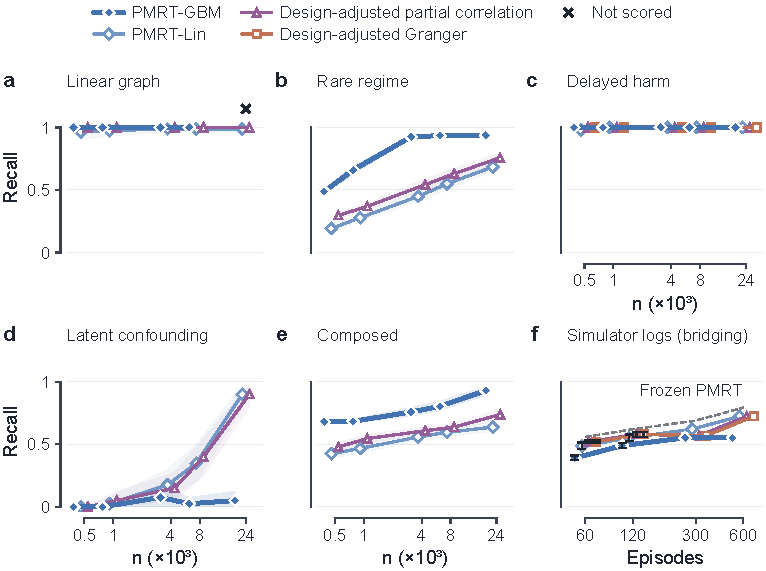
\includegraphics[width=\textwidth]{figures/fig_study4_recall.pdf}
\caption{Recall against sample size.}
\label{fig:s_recall}
\end{figure}

\begin{table}
\caption{Truth-null rate by dither design.}
\label{tab:s_dose}
% tab_appC_x2: generated by oran-causal-figures (packages/figures/src/oran_causal/figures/figs/tab_appC_x2.py); do not edit.
% Sources: data/records/posthoc_x2_x3/extras_tables.json
% Post hoc check X2: dither width; exploratory, no verdict.
% Pooled truth-null raw p <= .05 rejection rates, R2 of E1-E3, n 1000 and 4000, 4800 candidate tests per design; mark = condition-validity label (* INVALID, unmarked VALID).
% The 0.10 column is the 20-block design (the Study 4 R2 design). -- : design-adjusted partial correlation is not testable at 5 setpoint blocks (rank-deficient design). NOTEARS / SHAP-DAG give no p-values (csv only).
% Needs \usepackage{booktabs}.
\footnotesize
\setlength{\tabcolsep}{4pt}
\begin{tabular}{@{}l c c c c c c@{}}
\toprule
 & \multicolumn{4}{c}{Dither width (20 setpoint blocks)} & \multicolumn{2}{c}{Setpoint blocks (width 0.10)} \\
\cmidrule(lr){2-5}\cmidrule(lr){6-7}
Method & 0.02 & 0.05 & 0.10 & 0.20 & 5 & 80 \\
\midrule
\multicolumn{7}{@{}l}{\textit{Design-based tests}} \\
\quad PMRT-GBM & 0.049 & 0.045 & 0.046 & 0.043 & 0.044 & 0.046 \\
\quad PMRT-Lin & 0.045 & 0.042 & 0.045 & 0.043 & 0.050 & 0.054 \\
\addlinespace
\multicolumn{7}{@{}l}{\textit{Design-adjusted tests}} \\
\quad Partial correlation & 0.048 & 0.049 & 0.048 & 0.048 & -- & 0.054 \\
\addlinespace
\multicolumn{7}{@{}l}{\textit{Design-blind methods}} \\
\quad Correlation & 0.823$^{\textstyle *}$ & 0.803$^{\textstyle *}$ & 0.754$^{\textstyle *}$ & 0.619$^{\textstyle *}$ & 0.873$^{\textstyle *}$ & 0.571$^{\textstyle *}$ \\
\quad Partial correlation & 0.496$^{\textstyle *}$ & 0.485$^{\textstyle *}$ & 0.419$^{\textstyle *}$ & 0.253$^{\textstyle *}$ & 0.431$^{\textstyle *}$ & 0.312$^{\textstyle *}$ \\
\bottomrule
\end{tabular}

\end{table}

\begin{table}
\caption{Null-edge rate under a misspecified design.}
\label{tab:s_misspec}
% tab_appC_x3: generated by oran-causal-figures (packages/figures/src/oran_causal/figures/figs/tab_appC_x3.py); do not edit.
% Sources: data/records/posthoc_x2_x3/extras_tables.json
% Post hoc check X3: misspecified design; exploratory, no verdict.
% Raw p <= .05 rejection rates; R2 truth-null edges of E1-E2 (n 1000, 2640 candidate tests per design), E4 R3 confounded null edge (lambda 1, n 1000, 60 tests: one edge per seed). Mark = condition-validity label (* INVALID, ~ INCONCLUSIVE, unmarked VALID). Told multipliers are told / true; 1 = the exact design.
% The caption states that this is a degradation curve, not evidence against C2a.
% Needs \usepackage{booktabs}.
\footnotesize
\setlength{\tabcolsep}{2pt}
\begin{tabular}{@{}l c c c c c c c@{}}
\toprule
\multicolumn{8}{@{}l}{\textit{Truth-null edges, dithered setpoint, linear graph and rare regime}} \\
 & \multicolumn{5}{c}{Told dither width ($\times$ true)} & \multicolumn{2}{c}{Told setpoint delay} \\
\cmidrule(lr){2-6}\cmidrule(lr){7-8}
Method & 0.5 & 0.8 & 1 & 1.25 & 2 & +2\,\% & +5\,\% \\
\midrule
\quad PMRT-GBM & 0.152$^{\textstyle *}$ & 0.079$^{\textstyle *}$ & 0.042 & 0.040 & 0.100$^{\textstyle *}$ & 0.046 & 0.062$^{\textstyle *}$ \\
\quad PMRT-Lin & 0.313$^{\textstyle *}$ & 0.109$^{\textstyle *}$ & 0.042 & 0.016 & 0.000 & 0.086$^{\textstyle *}$ & 0.228$^{\textstyle *}$ \\
\quad PMRT-Lin, confounder covariates & 0.306$^{\textstyle *}$ & 0.107$^{\textstyle *}$ & 0.041 & 0.012 & 0.000 & 0.086$^{\textstyle *}$ & 0.208$^{\textstyle *}$ \\
\quad Design-adjusted partial correlation & 0.044 & 0.044 & 0.044 & 0.044 & 0.044 & 0.058 & 0.086$^{\textstyle *}$ \\
\midrule
\multicolumn{8}{@{}l}{\textit{Confounded null edge, latent confounding, state-dependent policy ($\lambda = 1$)}} \\
 & \multicolumn{5}{c}{Told $\lambda$ ($\times$ true)} & & \\
\cmidrule(lr){2-6}
Method & 0.5 & 0.8 & 1 & 1.25 & 2 & & \\
\midrule
\quad PMRT-GBM & 0.033$^{\textstyle\sim}$ & 0.017 & 0.017 & 0.017 & 0.267$^{\textstyle *}$ &  &  \\
\quad PMRT-Lin & 0.000 & 0.017 & 0.050$^{\textstyle\sim}$ & 0.050$^{\textstyle\sim}$ & 0.167$^{\textstyle *}$ &  &  \\
\quad PMRT-Lin, confounder covariates & 0.000 & 0.033$^{\textstyle\sim}$ & 0.033$^{\textstyle\sim}$ & 0.050$^{\textstyle\sim}$ & 0.183$^{\textstyle *}$ &  &  \\
\quad Design-adjusted partial correlation & 0.033$^{\textstyle\sim}$ & 0.033$^{\textstyle\sim}$ & 0.033$^{\textstyle\sim}$ & 0.033$^{\textstyle\sim}$ & 0.033$^{\textstyle\sim}$ &  &  \\
\bottomrule
\end{tabular}

\end{table}

\FloatBarrier
\section{Bridging analysis}
\label{esm:bridge}

The methods of the controlled environments ran on the randomised simulator logs, with the PMRT of the simulator as a reference row; Table~\ref{tab:s_bridge} gives the pooled recall and the null rates per method and subsample.

\begin{table}
\caption{Bridging analysis on the randomised logs.}
\label{tab:s_bridge}
% tab_appB_bridge: generated by oran-causal-figures (packages/figures/src/oran_causal/figures/figs/tab_appB_bridge.py); do not edit.
% Sources: data/records/bridging/exp_b/exp_b_tables.json
% Bridging analysis on the simulator logs of Studies 1-3: post hoc, descriptive, no verdict (EXP_B s.9).
% Rule: BY = Benjamini-Yekutieli at q .05; Plac. = placebo-calibrated threshold (leave one slice out; in-sample for pooled and the placebo logs). Rates are shares of hypotheses; slices 60 / 120 / 300 episodes and pooled (all 600). GT-NULL is an equivalence label, not a sharp null. Data sets = measure data sets with a record (of 72); dagger = partial coverage (MSCR: n <= 1000 only; CDD O-RAN discovery: 12 units over the CPU budget), not comparable with full-coverage rows. Slice-cluster CIs (2-10 clusters) stay in the source, not here. Left out (no paper name): pc_eq, mscr_eq.
% The frozen PMRT row is the reference (Studies 1-3 primary), not a competitor.
% Needs \usepackage{booktabs}.
\footnotesize
\setlength{\tabcolsep}{1pt}
\begin{tabular}{@{}l c c c c c c c c c c c c@{}}
\toprule
 & & Data & \multicolumn{4}{c}{Recall} & \multicolumn{4}{c}{Null rate} & Placebo & Placebo \\
\cmidrule(lr){4-7}\cmidrule(lr){8-11}
Method & Rule & sets & 60 & 120 & 300 & All & 60 & 120 & 300 & All & column & logs \\
\midrule
PMRT of the simulator (reference) & & & 0.56 & 0.62 & 0.69 & 0.79 & 0.10 & 0.10 & 0.10 & 0.10 &  & 0.00 \\
\midrule
\multicolumn{13}{@{}l}{\textit{Design-based tests}} \\
\quad PMRT-GBM & BY & 72 & 0.39 & 0.49 & 0.55 & 0.55 & 0.05 & 0.05 & 0.07 & 0.14 & 0.00 & 0.00 \\
\quad PMRT-Lin & BY & 72 & 0.49 & 0.55 & 0.62 & 0.72 & 0.05 & 0.06 & 0.10 & 0.10 & 0.00 & 0.00 \\
\quad PMRT-Lin, confounder covariates & BY & 72 & 0.49 & 0.55 & 0.59 & 0.72 & 0.05 & 0.07 & 0.10 & 0.10 & 0.00 & 0.00 \\
\midrule
\multicolumn{13}{@{}l}{\textit{Design-adjusted tests}} \\
\quad Partial correlation & BY & 72 & 0.52 & 0.58 & 0.57 & 0.72 & 0.05 & 0.06 & 0.10 & 0.10 & 0.00 & 0.00 \\
\quad Granger & BY & 72 & 0.52 & 0.58 & 0.57 & 0.72 & 0.05 & 0.06 & 0.10 & 0.10 & 0.00 & 0.00 \\
\quad RCoT & BY & 72 & 0.38 & 0.41 & 0.48 & 0.48 & 0.05 & 0.07 & 0.07 & 0.10 & 0.01 & 0.03 \\
\midrule
\multicolumn{13}{@{}l}{\textit{Design-blind methods}} \\
\quad Correlation & BY & 72 & 0.61 & 0.73 & 0.79 & 0.83 & 0.51 & 0.58 & 0.62 & 0.62 & 0.59 & 0.17 \\
\quad Partial correlation & BY & 72 & 0.52 & 0.58 & 0.57 & 0.69 & 0.05 & 0.06 & 0.10 & 0.10 & 0.00 & 0.00 \\
\quad Partial correlation, HAC (fixed-b) & BY & 72 & 0.52 & 0.57 & 0.57 & 0.69 & 0.05 & 0.06 & 0.10 & 0.10 & 0.00 & 0.00 \\
\quad Granger & BY & 72 & 0.62 & 0.70 & 0.74 & 0.76 & 0.41 & 0.55 & 0.69 & 0.76 & 0.40 & 0.22 \\
\quad RCoT & BY & 72 & 0.38 & 0.46 & 0.50 & 0.48 & 0.05 & 0.05 & 0.14 & 0.10 & 0.01 & 0.05 \\
\quad MSCR ($n \le 1000$, partial) & BY & 15 & 0.61 & 0.80 & -- & -- & 1.00 & 1.00 & -- & -- & 0.56 & 0.33 \\
\quad Two-tower & Plac. & 72 & 0.27 & 0.29 & 0.22 & 0.34 & 0.10 & 0.10 & 0.07 & 0.10 & 0.05 & 0.15 \\
\quad CDD O-RAN discovery (partial) & Plac. & 60 & 0.40 & 0.49 & 0.44 & 0.25 & 0.08 & 0.23 & 1.00 & 1.00 & 0.05 & 0.05 \\
\quad PC & Plac. & 72 & 0.11 & 0.12 & 0.19 & 0.14 & 0.10 & 0.06 & 0.14 & 0.14 & 0.05 & 0.07 \\
\quad NOTEARS & Plac. & 72 & 0.19 & 0.20 & 0.22 & 0.24 & 0.05 & 0.05 & 0.05 & 0.05 & 0.01 & 0.05 \\
\quad SHAP-DAG & Plac. & 72 & 0.27 & 0.26 & 0.33 & 0.28 & 0.07 & 0.07 & 0.05 & 0.05 & 0.04 & 0.00 \\
\bottomrule
\end{tabular}

\end{table}

\FloatBarrier
\end{document}
